%!TEX program = xelatex
\documentclass[UTF8,zihao=5]{ctexart} %ctex包的article


\usepackage[hidelinks]{hyperref}%超链接,自动加到目录里面



\title{{\bfseries\rmfamily\Huge{高等流体力学\hspace{1em}\\第2次作业}}}
\author{周涵宇 2022310984}
\date{}

\usepackage[a4paper]{geometry}
\geometry{left=0.75in,right=0.75in,top=1in,bottom=1in}%纸张大小和页边距

\usepackage[
UseMSWordMultipleLineSpacing,
MSWordLineSpacingMultiple=1.5
]{zhlineskip}%office风格的行间距

\usepackage{fontspec}
\setmainfont{Times New Roman}
\setsansfont{Source Sans Pro}
\setmonofont{Latin Modern Mono}
\setCJKmainfont{SimSun}[AutoFakeBold=true]
% \setCJKmainfont{仿宋}[AutoFakeBold=true]
\setCJKsansfont{黑体}[AutoFakeBold=true]
\setCJKmonofont{DengXian}[AutoFakeBold=true]

\setCJKfamilyfont{kaiti}{楷体}
\newfontfamily\CM{Cambria Math}


% \usepackage{indentfirst} %不工作 怎样调整ctex的段首缩进大小呢

\usepackage{fancyhdr}
\pagestyle{fancy}
\lhead{
    \CJKfamily{kaiti}{
        高等流体力学作业\hspace{6em}
        班级\ \ 航博221\hspace{6em}
        学号\ \ 2022310984\hspace{6em}
        姓名\ \ 周涵宇
        }
}
\chead{}
\rhead{}
\lfoot{}
\cfoot{\thepage}
\rfoot{}
\renewcommand{\headrulewidth}{0.5pt} %改为0pt即可去掉页眉下面的横线
\renewcommand{\footrulewidth}{0pt} %改为0pt即可去掉页脚上面的横线
\setcounter{page}{1}


% \usepackage{bm}

\usepackage{amsmath,amsfonts}
\usepackage{array}
\usepackage{enumitem}
\usepackage{unicode-math}

% \usepackage{titlesec} % it subverts the ctex titles
\usepackage{titletoc}


% titles in toc:
\titlecontents{section}
              [2cm]
              {\sffamily\zihao{5}\mdseries}%
              {\contentslabel{3em}}%
              {}%
              {\titlerule*[0.5pc]{-}\contentspage\hspace*{1cm}}

\titlecontents{subsection}
              [3cm]
              {\rmfamily\mdseries\zihao{5}}%
              {\contentslabel{3em}}%
              {}%
              {\titlerule*[0.5pc]{-}\contentspage\hspace*{1cm}}

\titlecontents{subsubsection}
              [4cm]
              {\rmfamily\mdseries\zihao{5}}%
              {\contentslabel{3em}}%
              {}%
              {\titlerule*[0.5pc]{-}\contentspage\hspace*{1cm}}
\renewcommand*\contentsname{\hfill \sffamily\mdseries 目录 \hfill}

\ctexset{
    section={   
        % name={前面,后面},
        number={\arabic{section}.},
        format=\sffamily\raggedright\zihao{4}\mdseries,
        indent= {0em},
        aftername = \hspace{0.5em},
        beforeskip=1ex,
        afterskip=1ex
    },
    subsection={   
        % name={另一个前面,另一个后面},
        number={\arabic{section}.\arabic{subsection}.}, %如果只用一个数字而非1.1
        format=\rmfamily\raggedright\mdseries\zihao{5},%正体字体,不加粗,main字体,五号字
        indent = {2em}, %缩进
        aftername = \hspace{0.5em},
        beforeskip=1ex,
        afterskip=1ex
    },
    subsubsection={   
        % name={另一个前面,另一个后面},
        number={\arabic{section}.\arabic{subsection}.\arabic{subsubsection}.}, %默认的 1.1.1
        format=\rmfamily\raggedright\mdseries\zihao{5},%无衬线字体,加粗,sans字体,五号字
        indent = {2em}, %缩进
        aftername = \hspace{0.5em},  %名字和标题间插入字符(此处是空白)
        beforeskip=1ex, %空行
        afterskip=1ex
    }
}

\usepackage{float}
\usepackage{graphicx}
\usepackage{multirow}
\usepackage{multicol}
\usepackage{caption}
\usepackage{subcaption}


%part、section、subsection、subsubsection、paragraph、subparagraph
\newcommand{\bm}[1]{{\mathbf{#1}}}
\newcommand{\trans}[0]{^\mathrm{T}}
\newcommand{\tran}[1]{#1^\mathrm{T}}
\newcommand{\hermi}[0]{^\mathrm{H}}
\newcommand{\conj}[1]{\overline{#1}}
\newcommand*{\av}[1]{\left\langle{#1}\right\rangle}
\newcommand*{\avld}[1]{\frac{\overline{D}#1}{Dt}}
\newcommand*{\pd}[2]{\frac{\partial #1}{\partial #2}}
\newcommand*{\pdcd}[3]{\frac{\partial^2 #1}{\partial #2 \partial #3}}
\newcommand*{\inc}[0]{{\Delta}}

\newcommand*{\uu}[0]{\bm{u}}
\newcommand*{\vv}[0]{\bm{v}}
\newcommand*{\g}[0]{\bm{g}}
\newcommand*{\nb}[0]{{\nabla}}



\begin{document}

\maketitle
\thispagestyle{fancy}


% \begin{center}
%     \rmfamily
%     \tableofcontents\setcounter{page}{0}
% \end{center}
% \thispagestyle{empty} % 目录
% \newpage %换页

\section{线性稳定性分析}

是两个独立系统。

\subsection{}
考虑
$$
    \frac{dx}{dt} = \mu + x^2
$$
则有平衡点$\pm\sqrt{-\mu}$,在$\mu\leq 0$存在。
$$
    \frac{d(\mu + x^2)}{dx} = 2x
$$
则明显,若有两个平衡点,
当$+\sqrt{-\mu}$处为不稳定结点,而$-\sqrt{-\mu}$处为稳定结点;
若$\mu=0$,则$0$为平衡点,线性意义下中性稳定。

\subsection{}
考虑
$$
    \frac{dy}{dt}=\pm y
$$
则都只有$y=0$为平衡点,其特征值就是$\pm 1$,则取正号为不稳定结点,负号为稳定结点。

\label{sec:1}

\section{Lorenz 系统}

考虑
$$
    \begin{array}{rl}
        \frac{dX}{d\tau}  = & -\sigma X + \sigma Y \\
        \frac{dY}{d\tau}  = & rX - Y - XZ          \\
        \frac{dZ}{d\tau}  = & -bZ + XY             \\
    \end{array}
$$
取$\sigma = 10,\ b=8/3$,现数值研究不同$r$时的系统特性。

由于已知三个平衡点:
$$
    \begin{array}{l}
        X=Y=Z=0                        \\
        X=Y=\sqrt{b(r-1)} , \ Z = r-1  \\
        X=Y=-\sqrt{b(r-1)} , \ Z = r-1 \\
    \end{array}
$$
其中两个在$r>1$有意义。本文选取的初值都在平衡点附近,这样方便观察其行为。

求解ODE的方法为1-13阶变阶数Adams-Bashforth-Moulton方法,见
(Shampine, L. F. and M. K. Gordon, Computer Solution of Ordinary Differential Equations: the Initial Value Problem, W. H. Freeman, San Francisco, 1975)。
变阶数步长中的绝对、相对误差限都取$10^{-12}$。

根据文献(Steven H. Strogatz, Nonlinear Dynamics and Chaos: With Applications in Physics, Biology, Chemistry, and Engineering, Addison Wesley, 1994),
选取不同的$r$的范围进行计算。

\subsection{$r<1$}

选择$r=0.5$,不同初值计算,如下图
\begin{figure}[H]
    \begin{minipage}[c]{0.45\linewidth}  %需调整
        \centering
        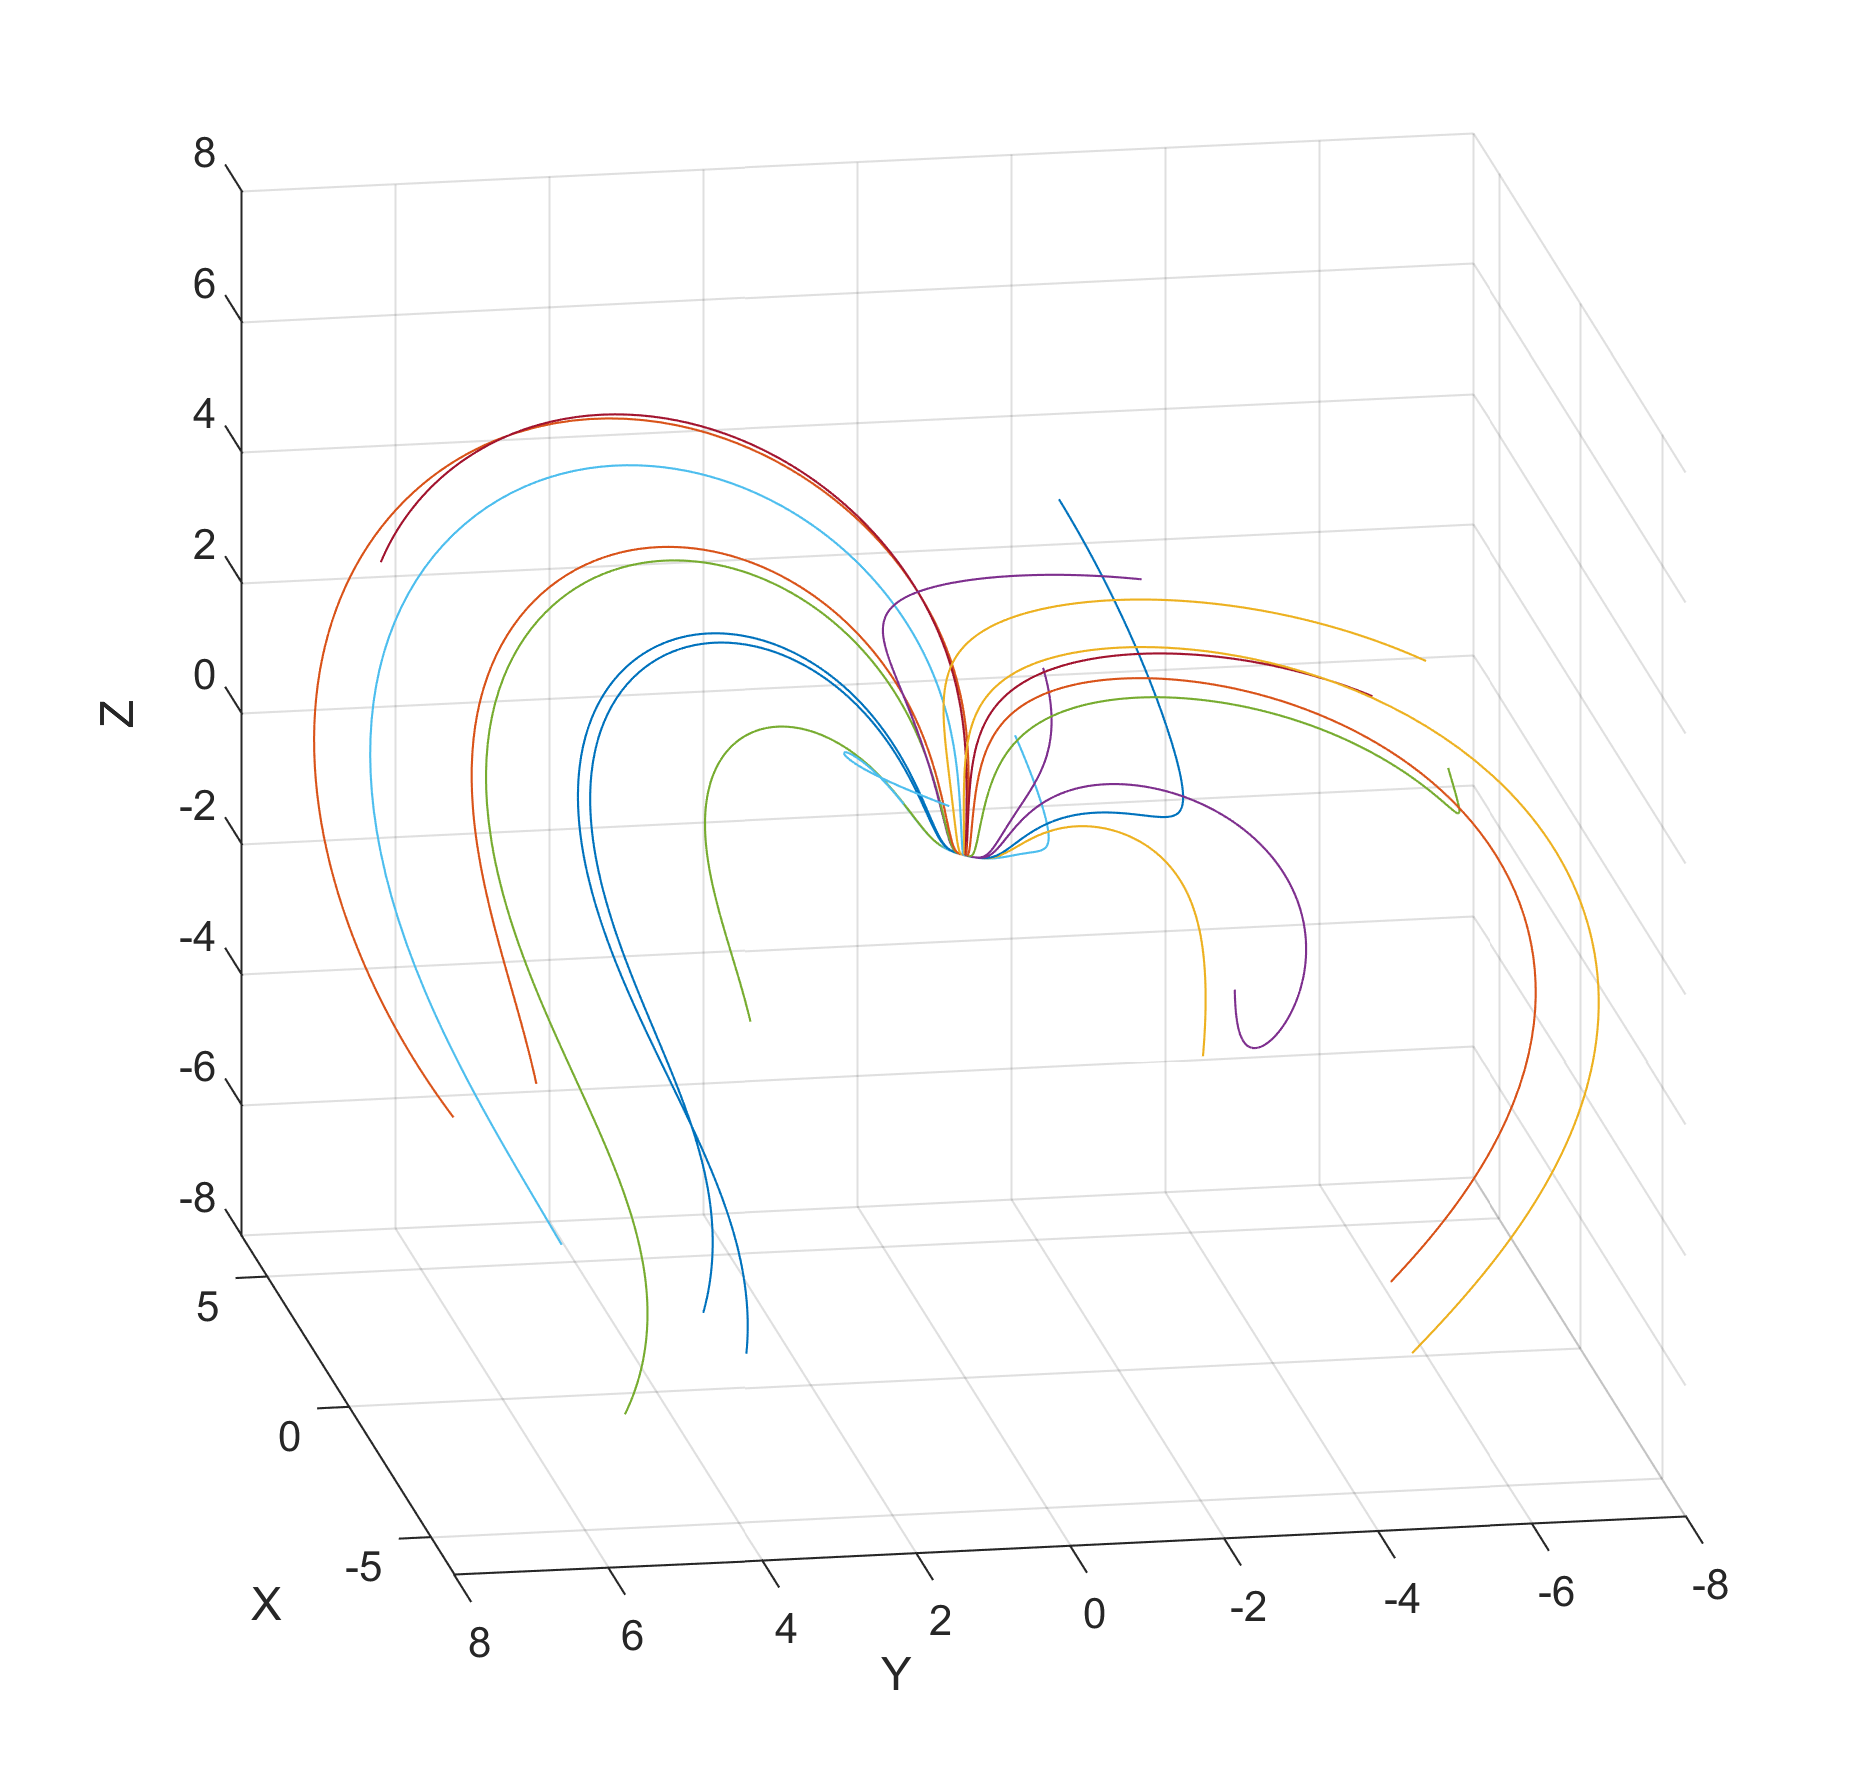
\includegraphics[width=8cm]{XYZ_r_0.5.png}  %需调整
        \caption{$r=0.5$,相空间轨迹}
    \end{minipage}
    \hfill %弹性长度
    \begin{minipage}[c]{0.45\linewidth}  %需调整
        \centering
        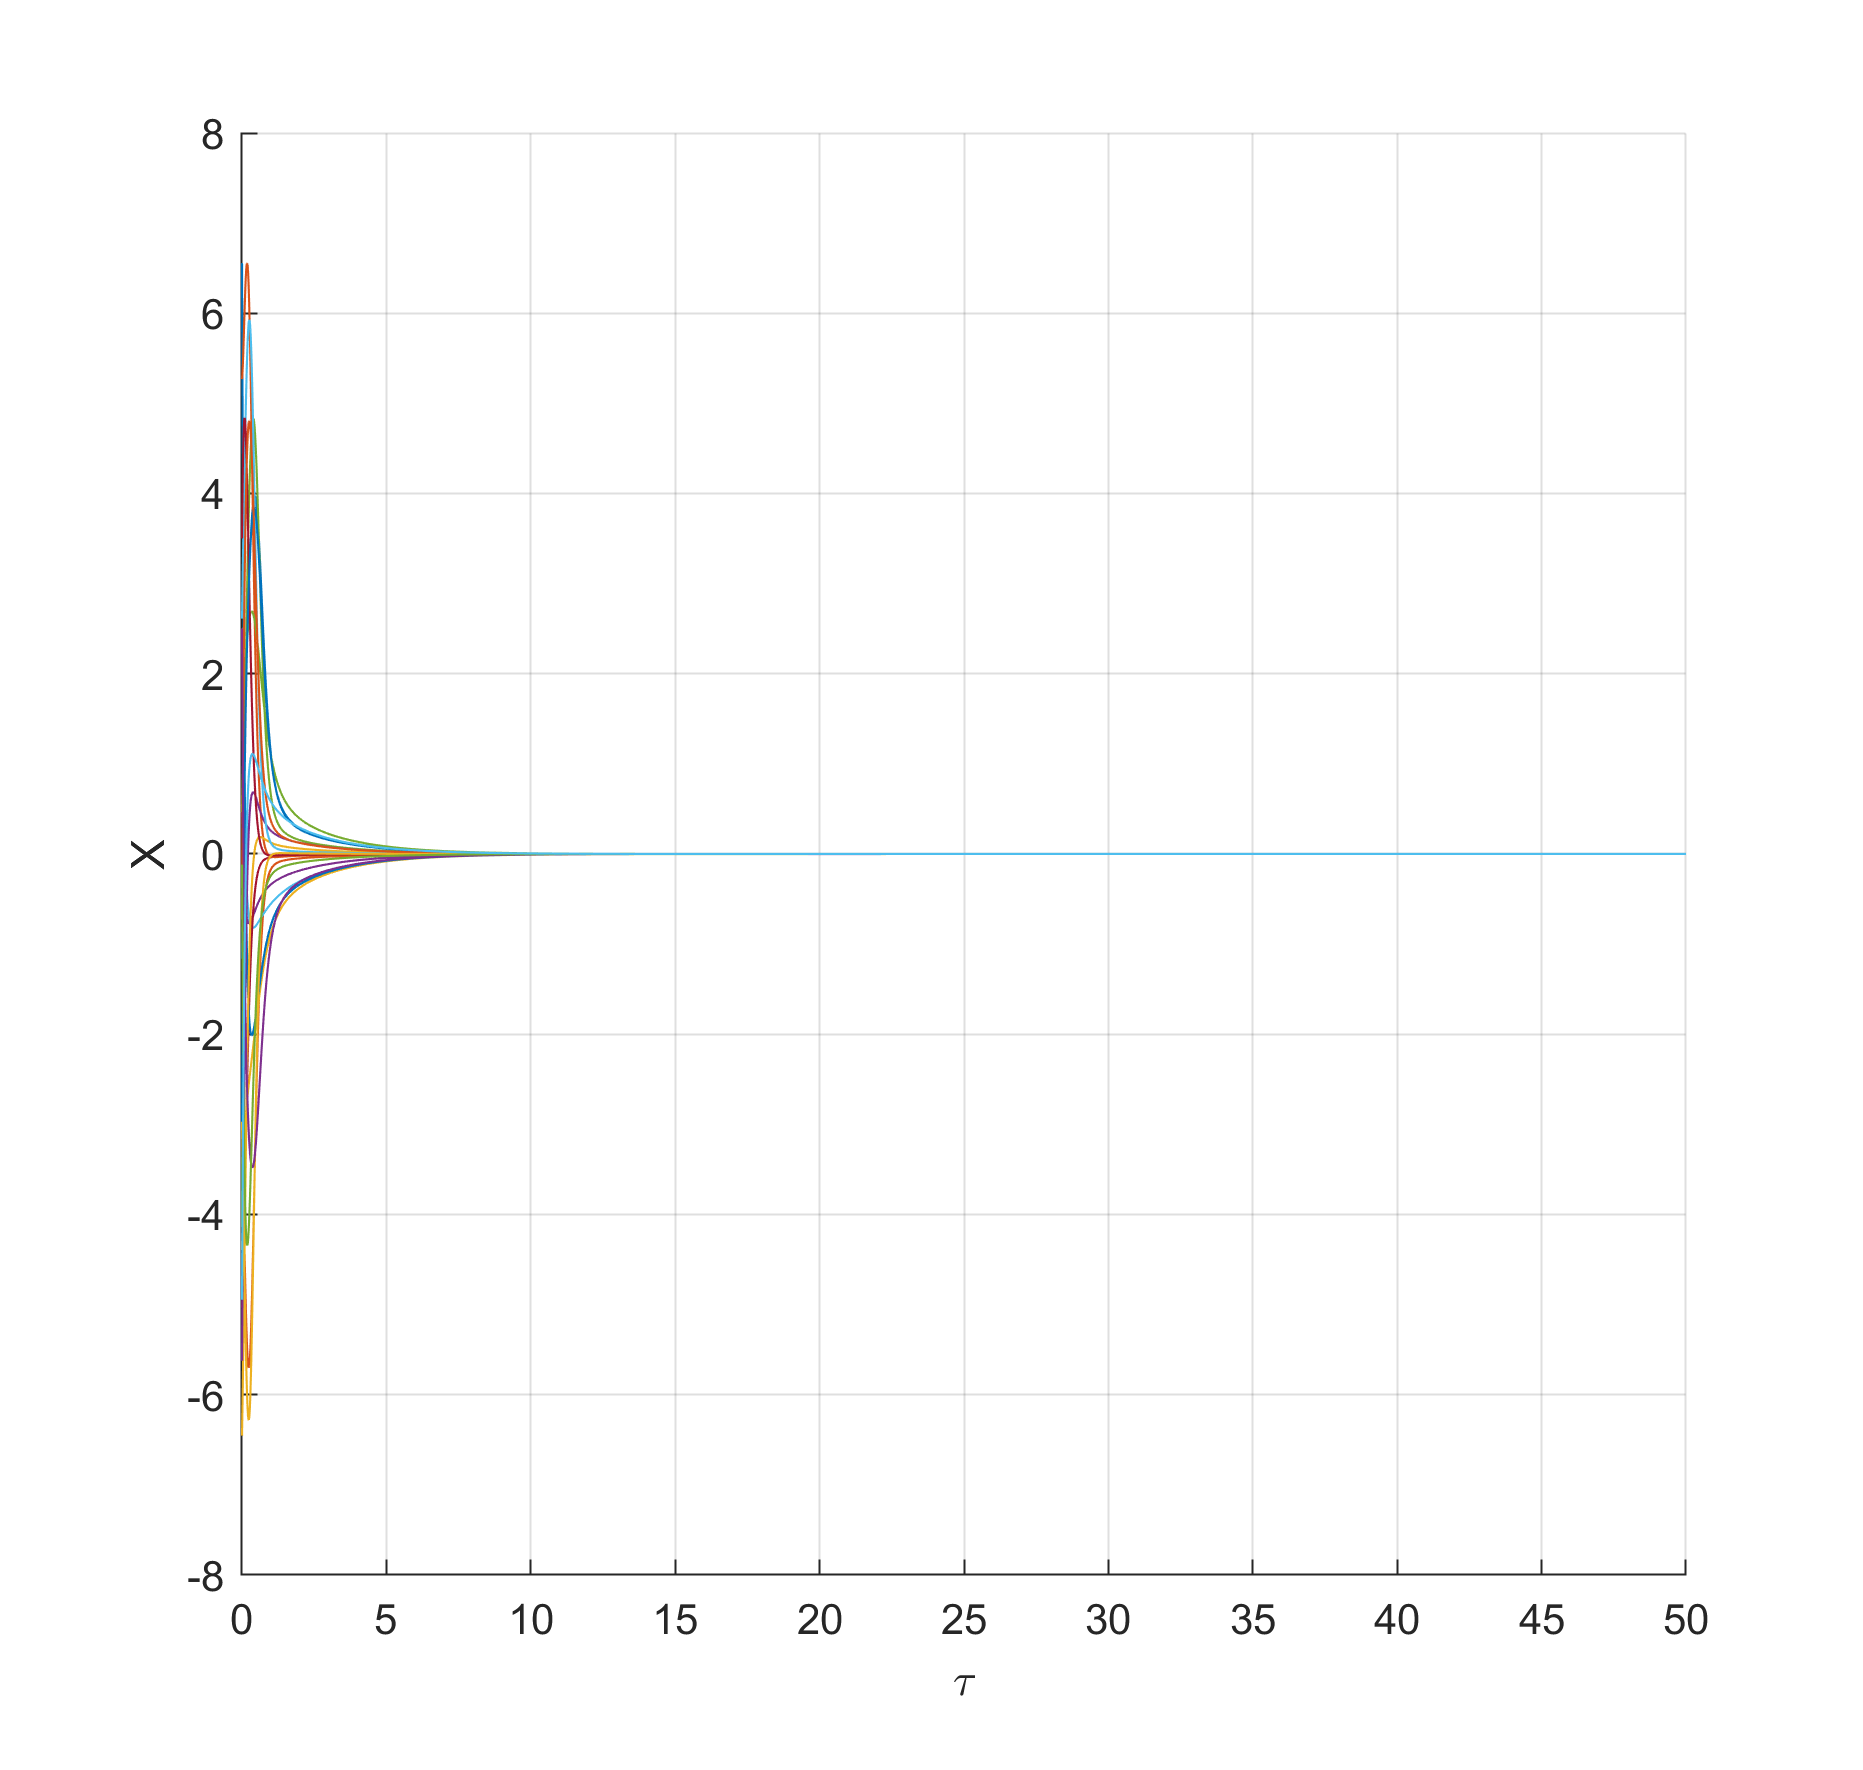
\includegraphics[width=8cm]{XT_r_0.5.png}  %需调整
        \caption{$r=0.5$,$X$沿时间变化}
    \end{minipage}
\end{figure}
可见原点是一个稳定的节点,解都快速衰减为0。

\subsection{$1<r<13.926$}

选择$r=1.3,2,8$,不同初值计算,如下图
\begin{figure}[H]
    \begin{minipage}[c]{0.45\linewidth}  %需调整
        \centering
        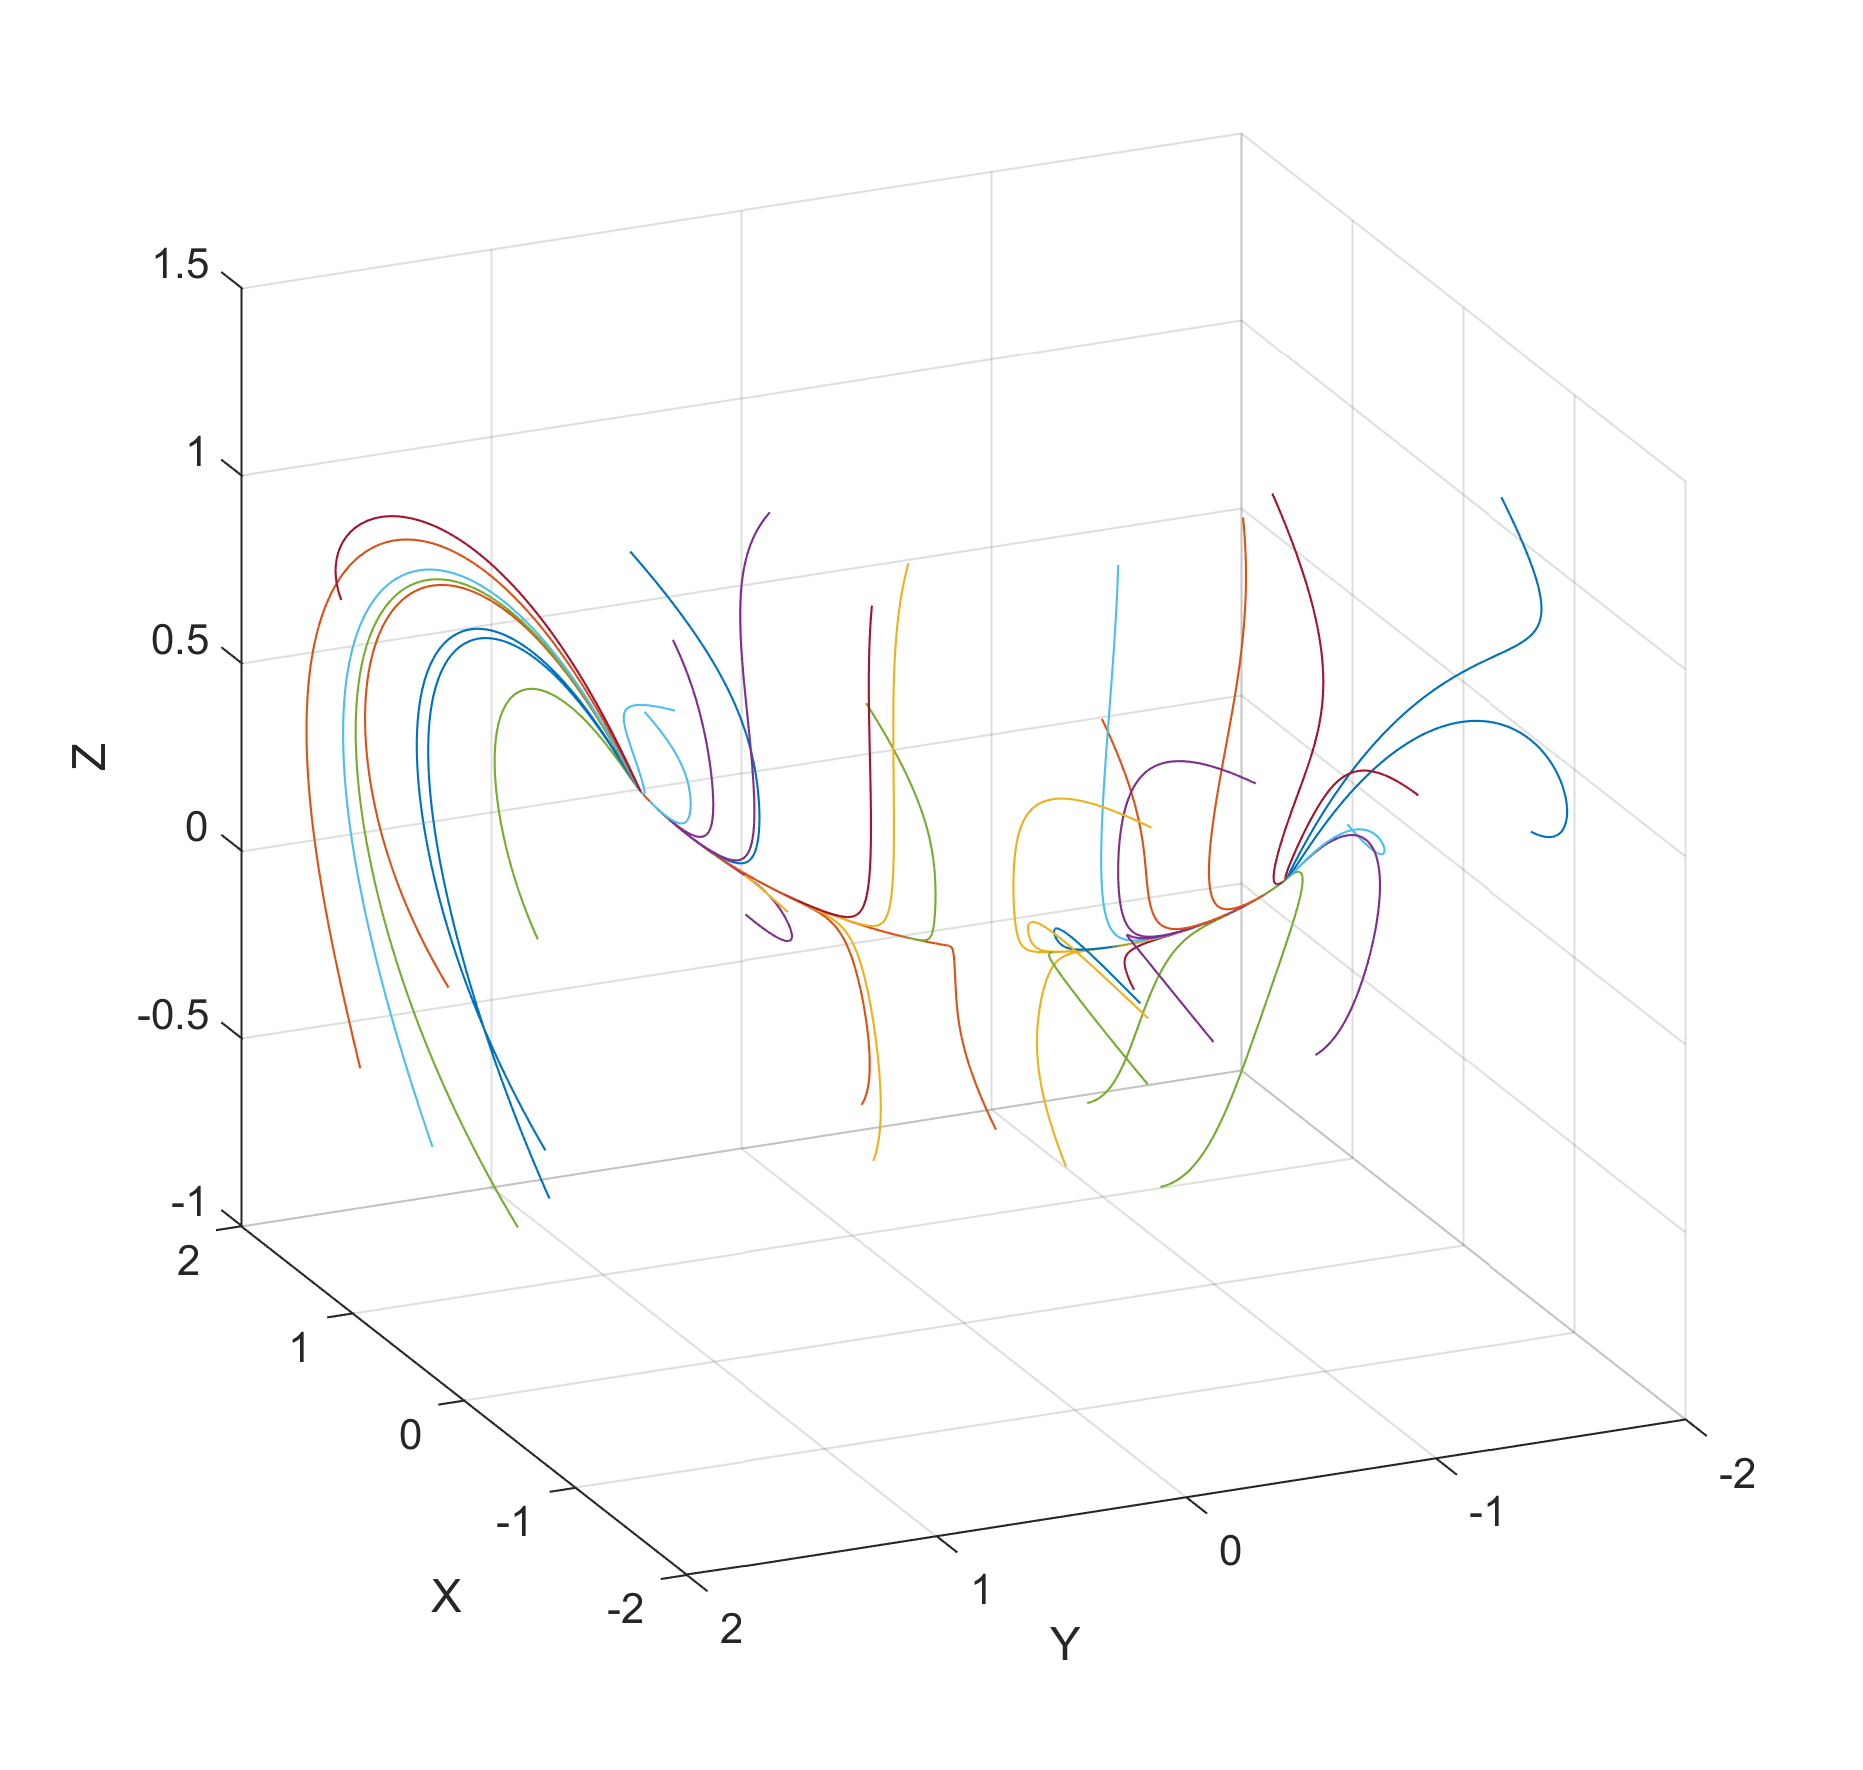
\includegraphics[width=8cm]{XYZ_r_1.3.png}  %需调整
        \caption{$r=1.3$,相空间轨迹}
    \end{minipage}
    \hfill %弹性长度
    \begin{minipage}[c]{0.45\linewidth}  %需调整
        \centering
        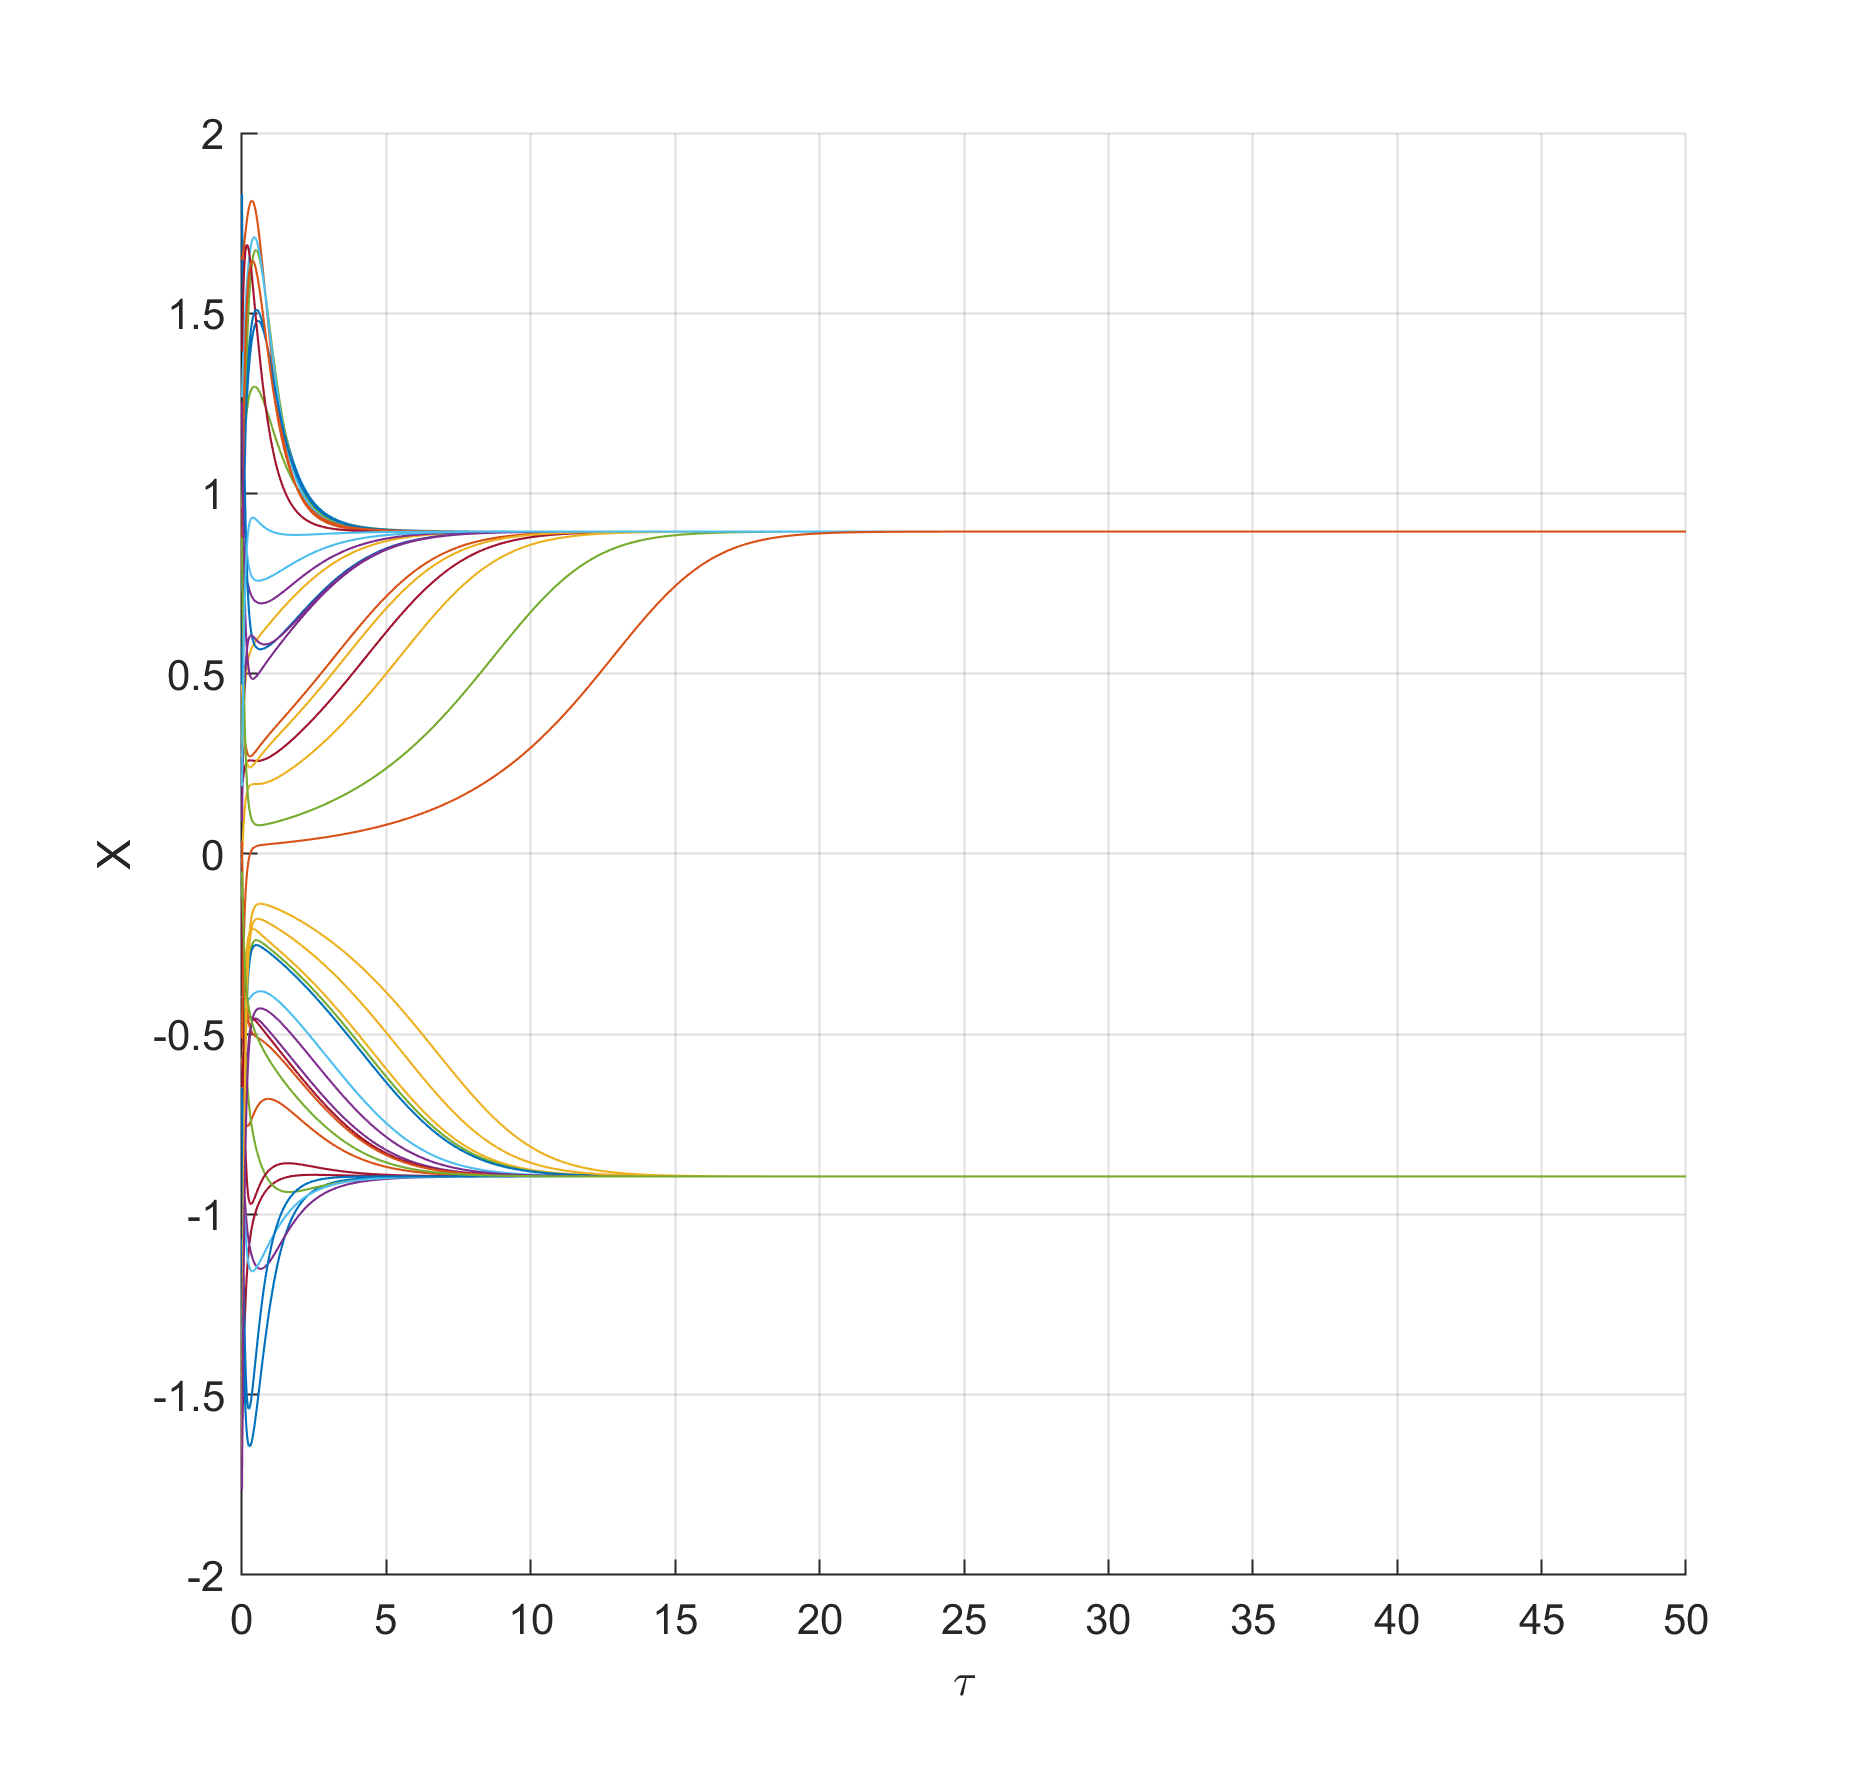
\includegraphics[width=8cm]{XT_r_1.3.png}  %需调整
        \caption{$r=1.3$,$X$沿时间变化}
    \end{minipage}
\end{figure}

\begin{figure}[H]
    \begin{minipage}[c]{0.45\linewidth}  %需调整
        \centering
        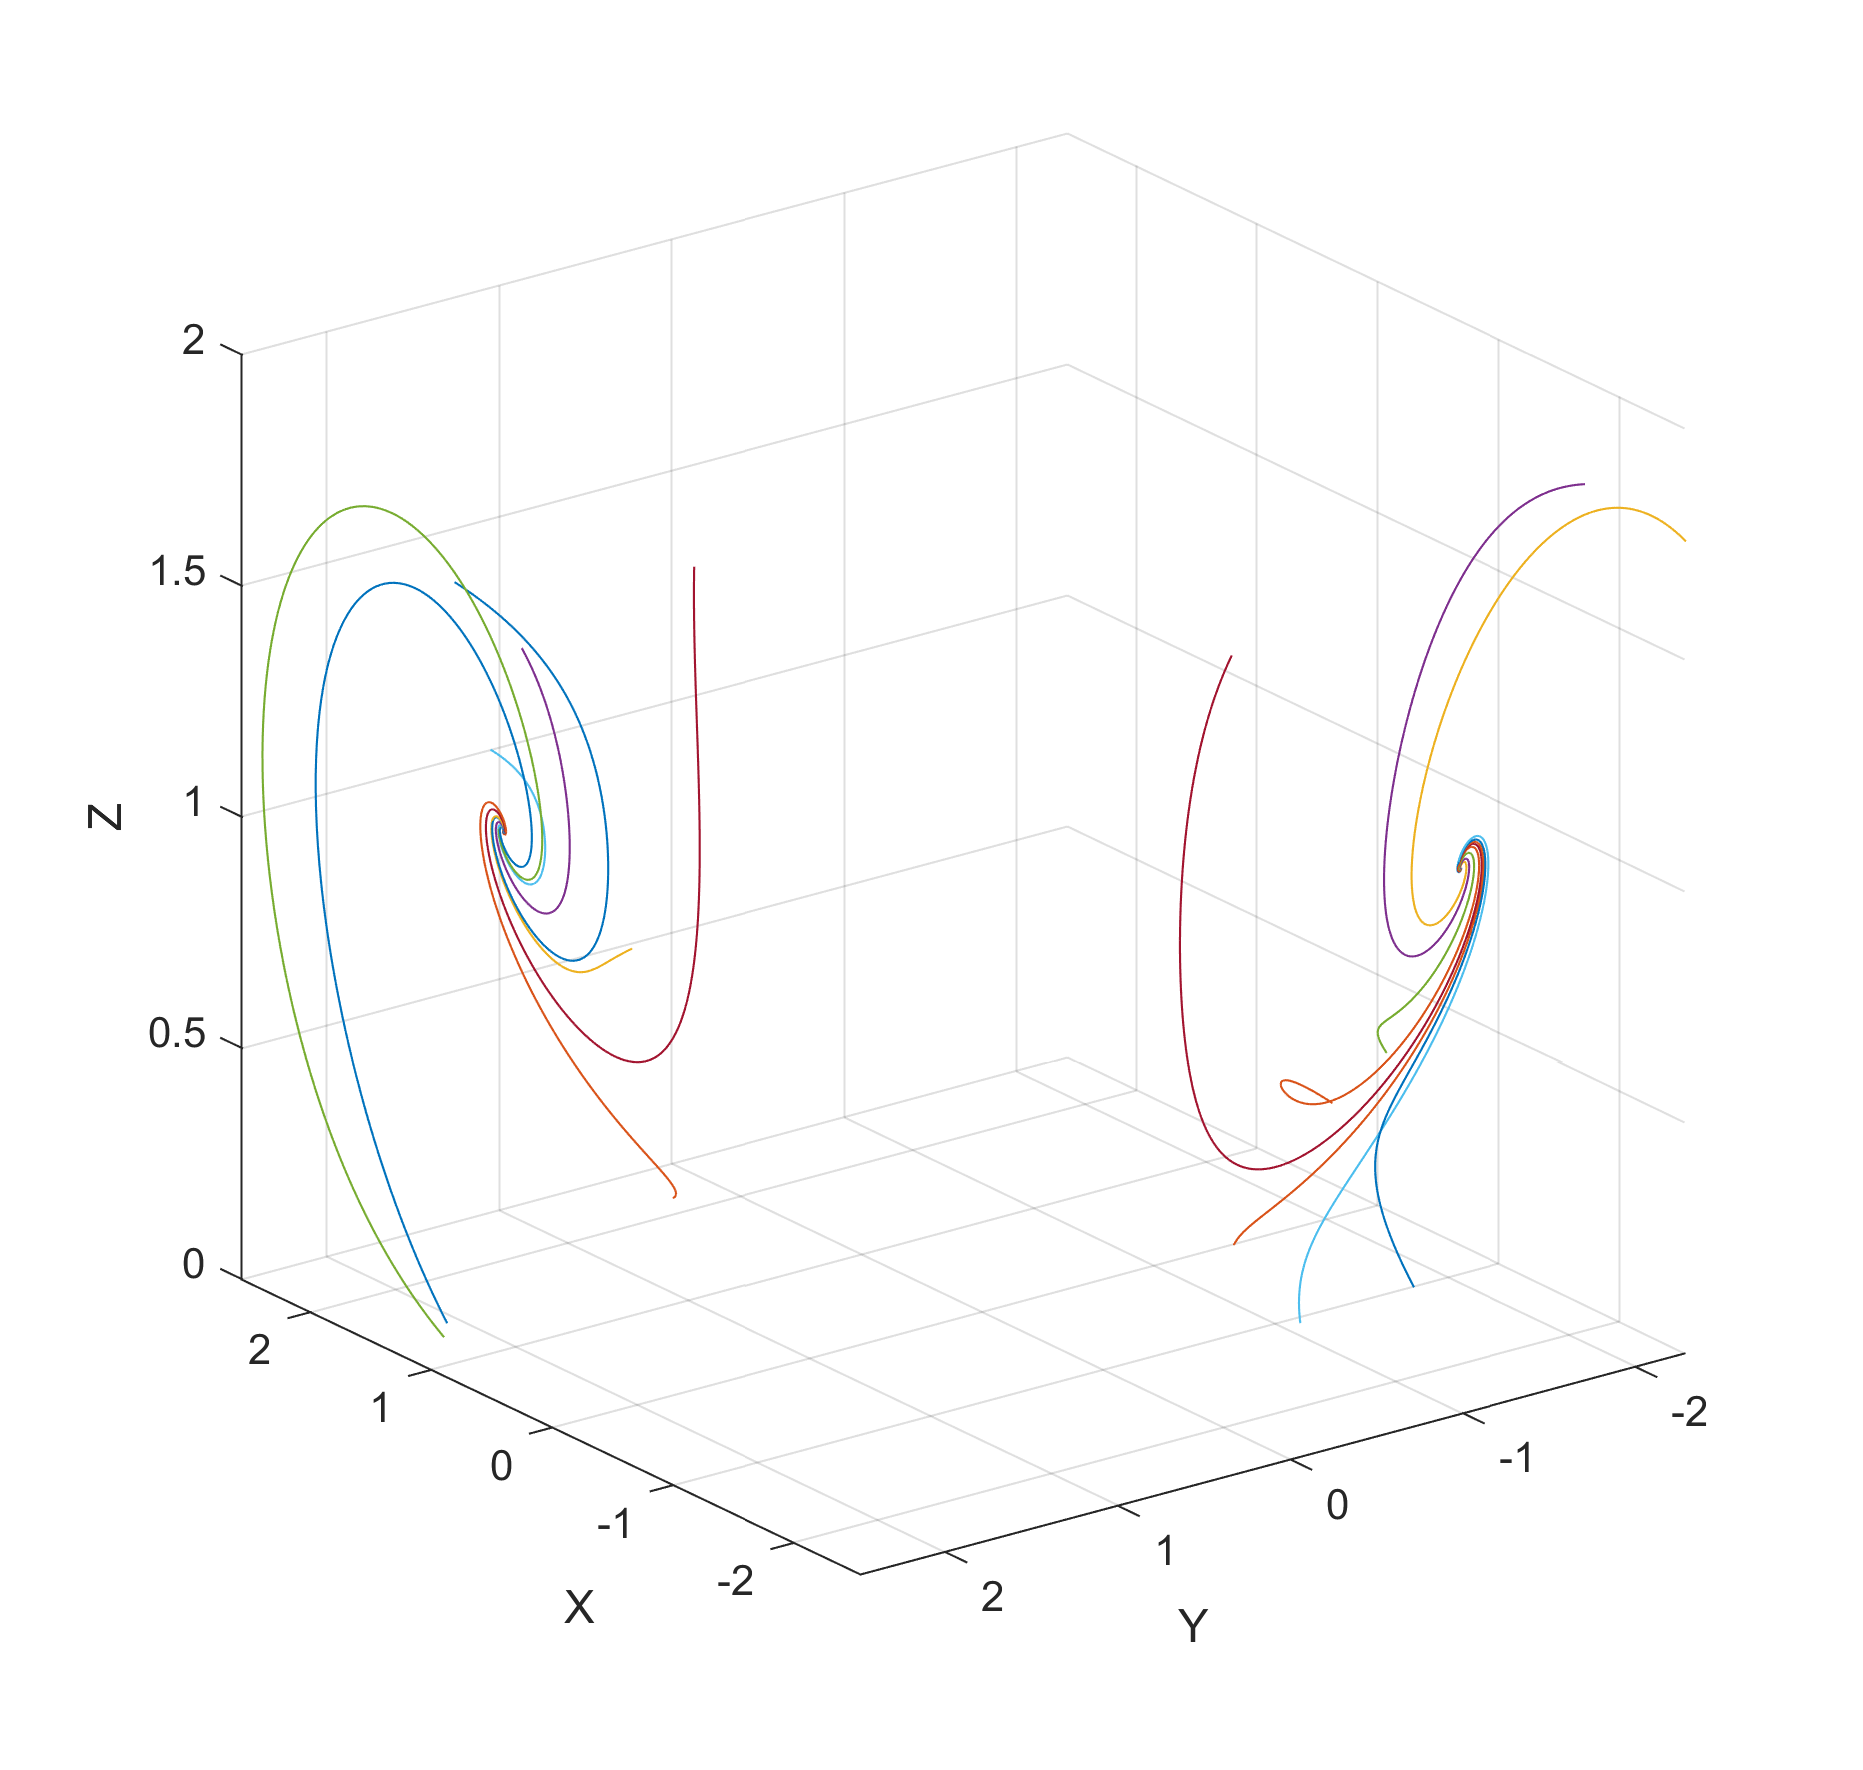
\includegraphics[width=8cm]{XYZ_r_2.png}  %需调整
        \caption{$r=2$,相空间轨迹}
    \end{minipage}
    \hfill %弹性长度
    \begin{minipage}[c]{0.45\linewidth}  %需调整
        \centering
        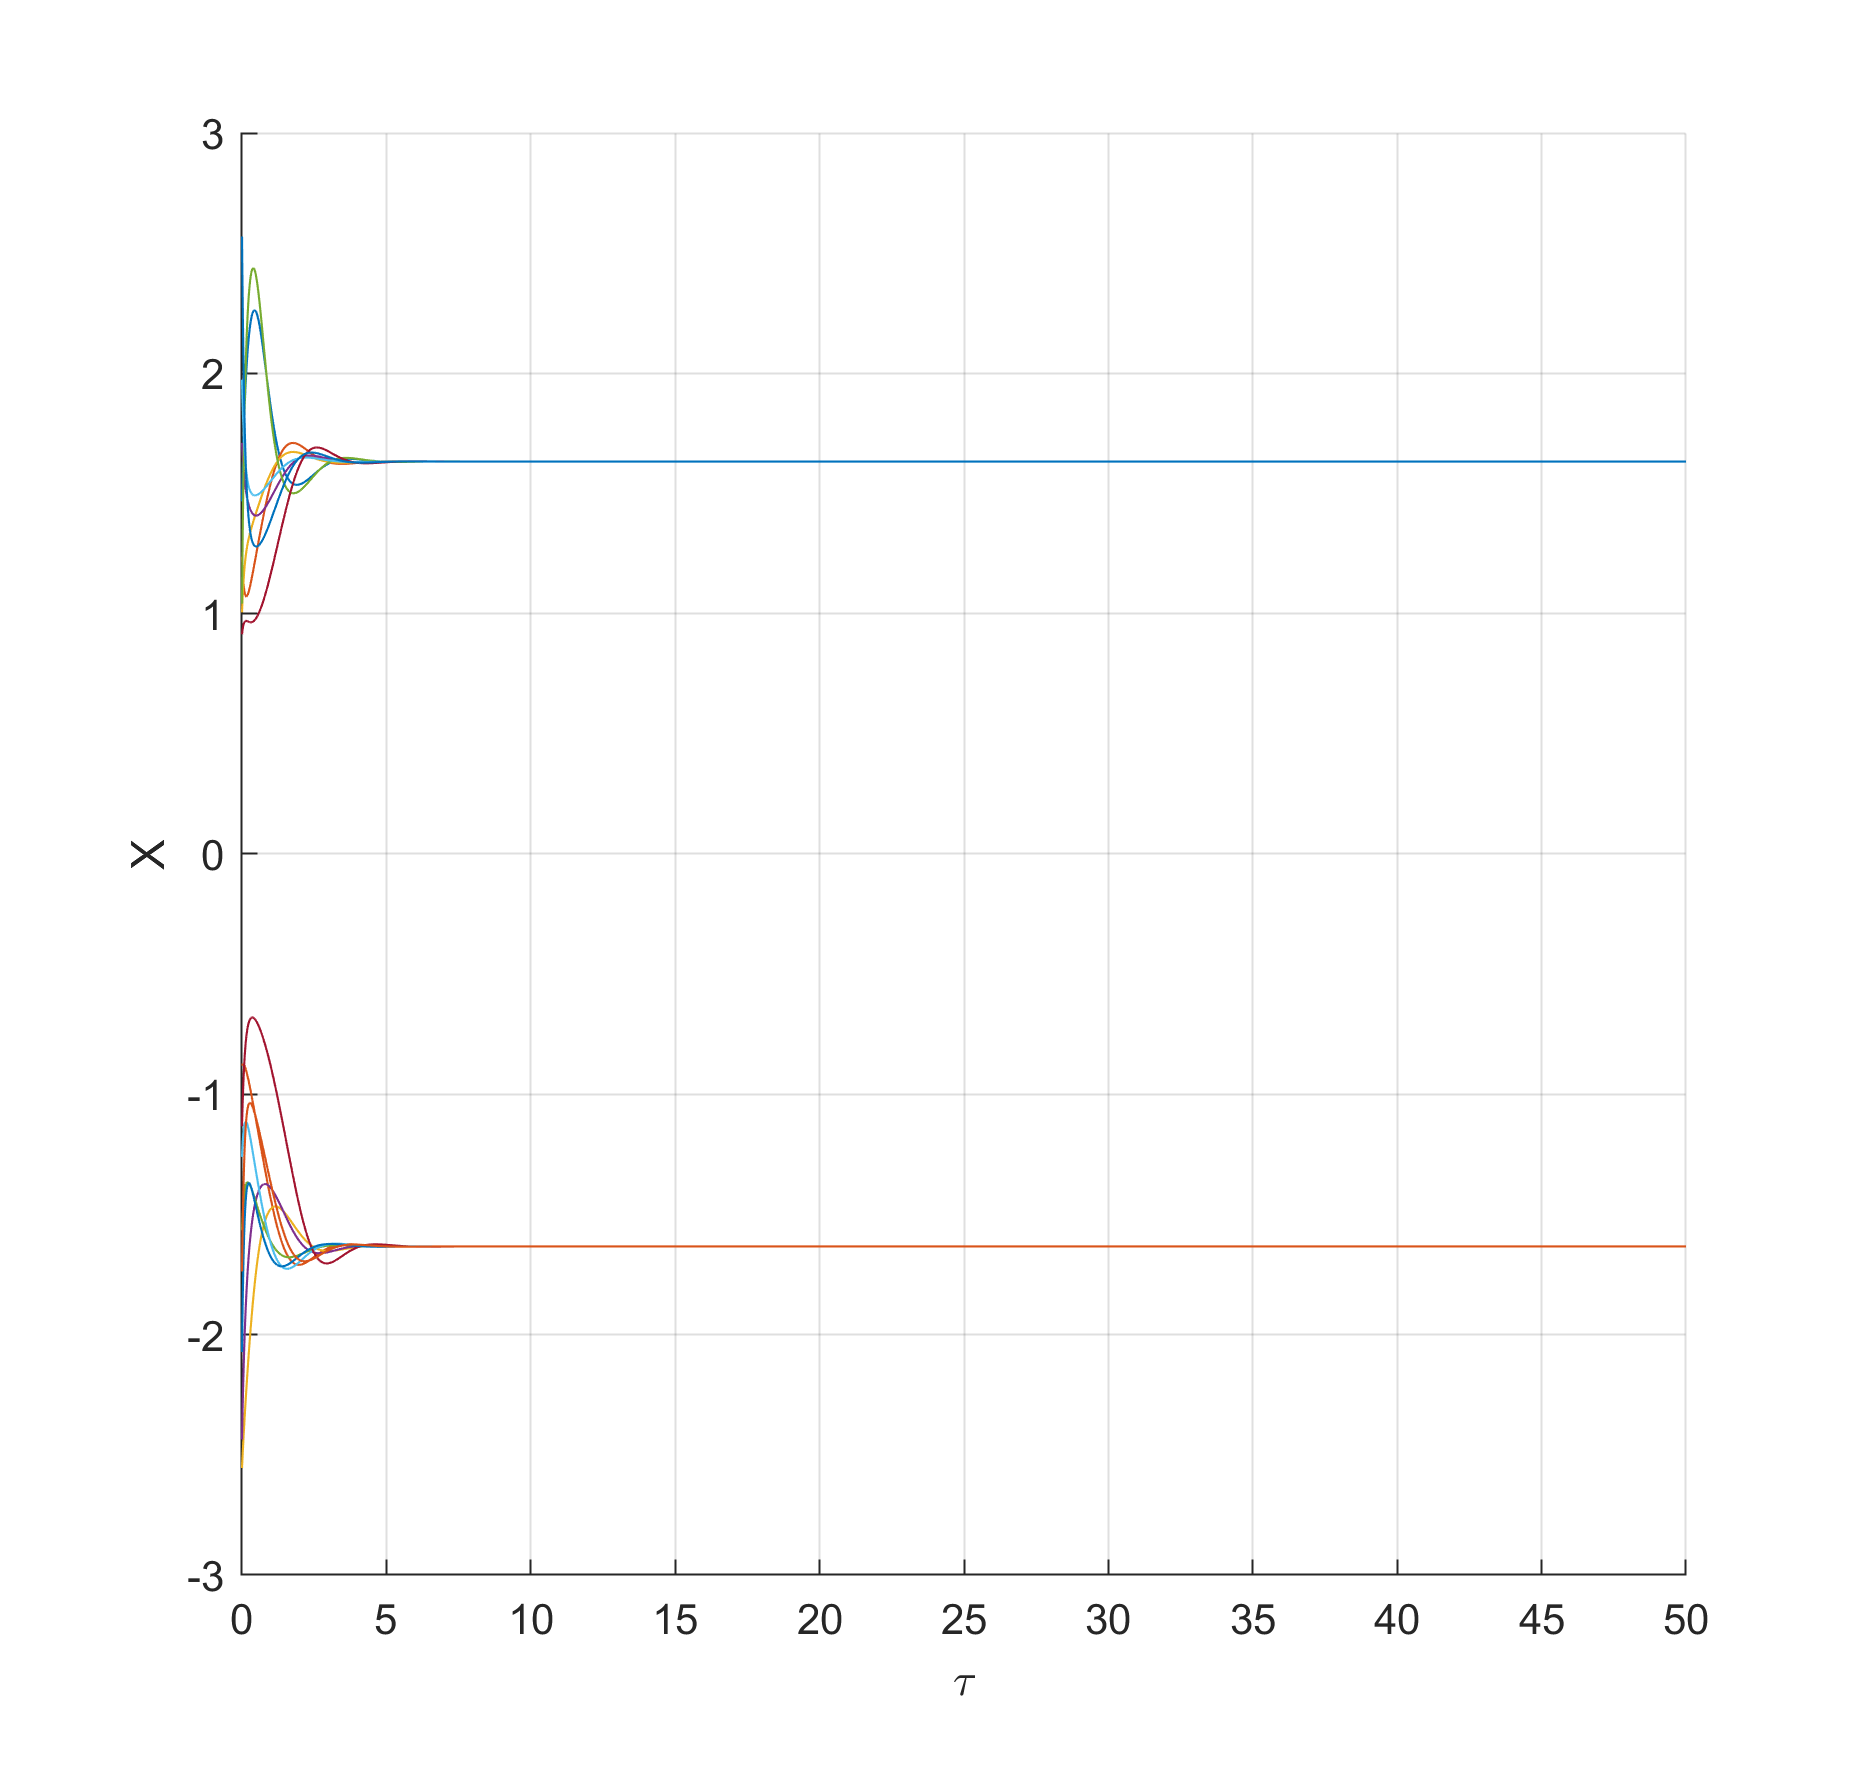
\includegraphics[width=8cm]{XT_r_2.png}  %需调整
        \caption{$r=2$,$X$沿时间变化}
    \end{minipage}
\end{figure}

\begin{figure}[H]
    \begin{minipage}[c]{0.45\linewidth}  %需调整
        \centering
        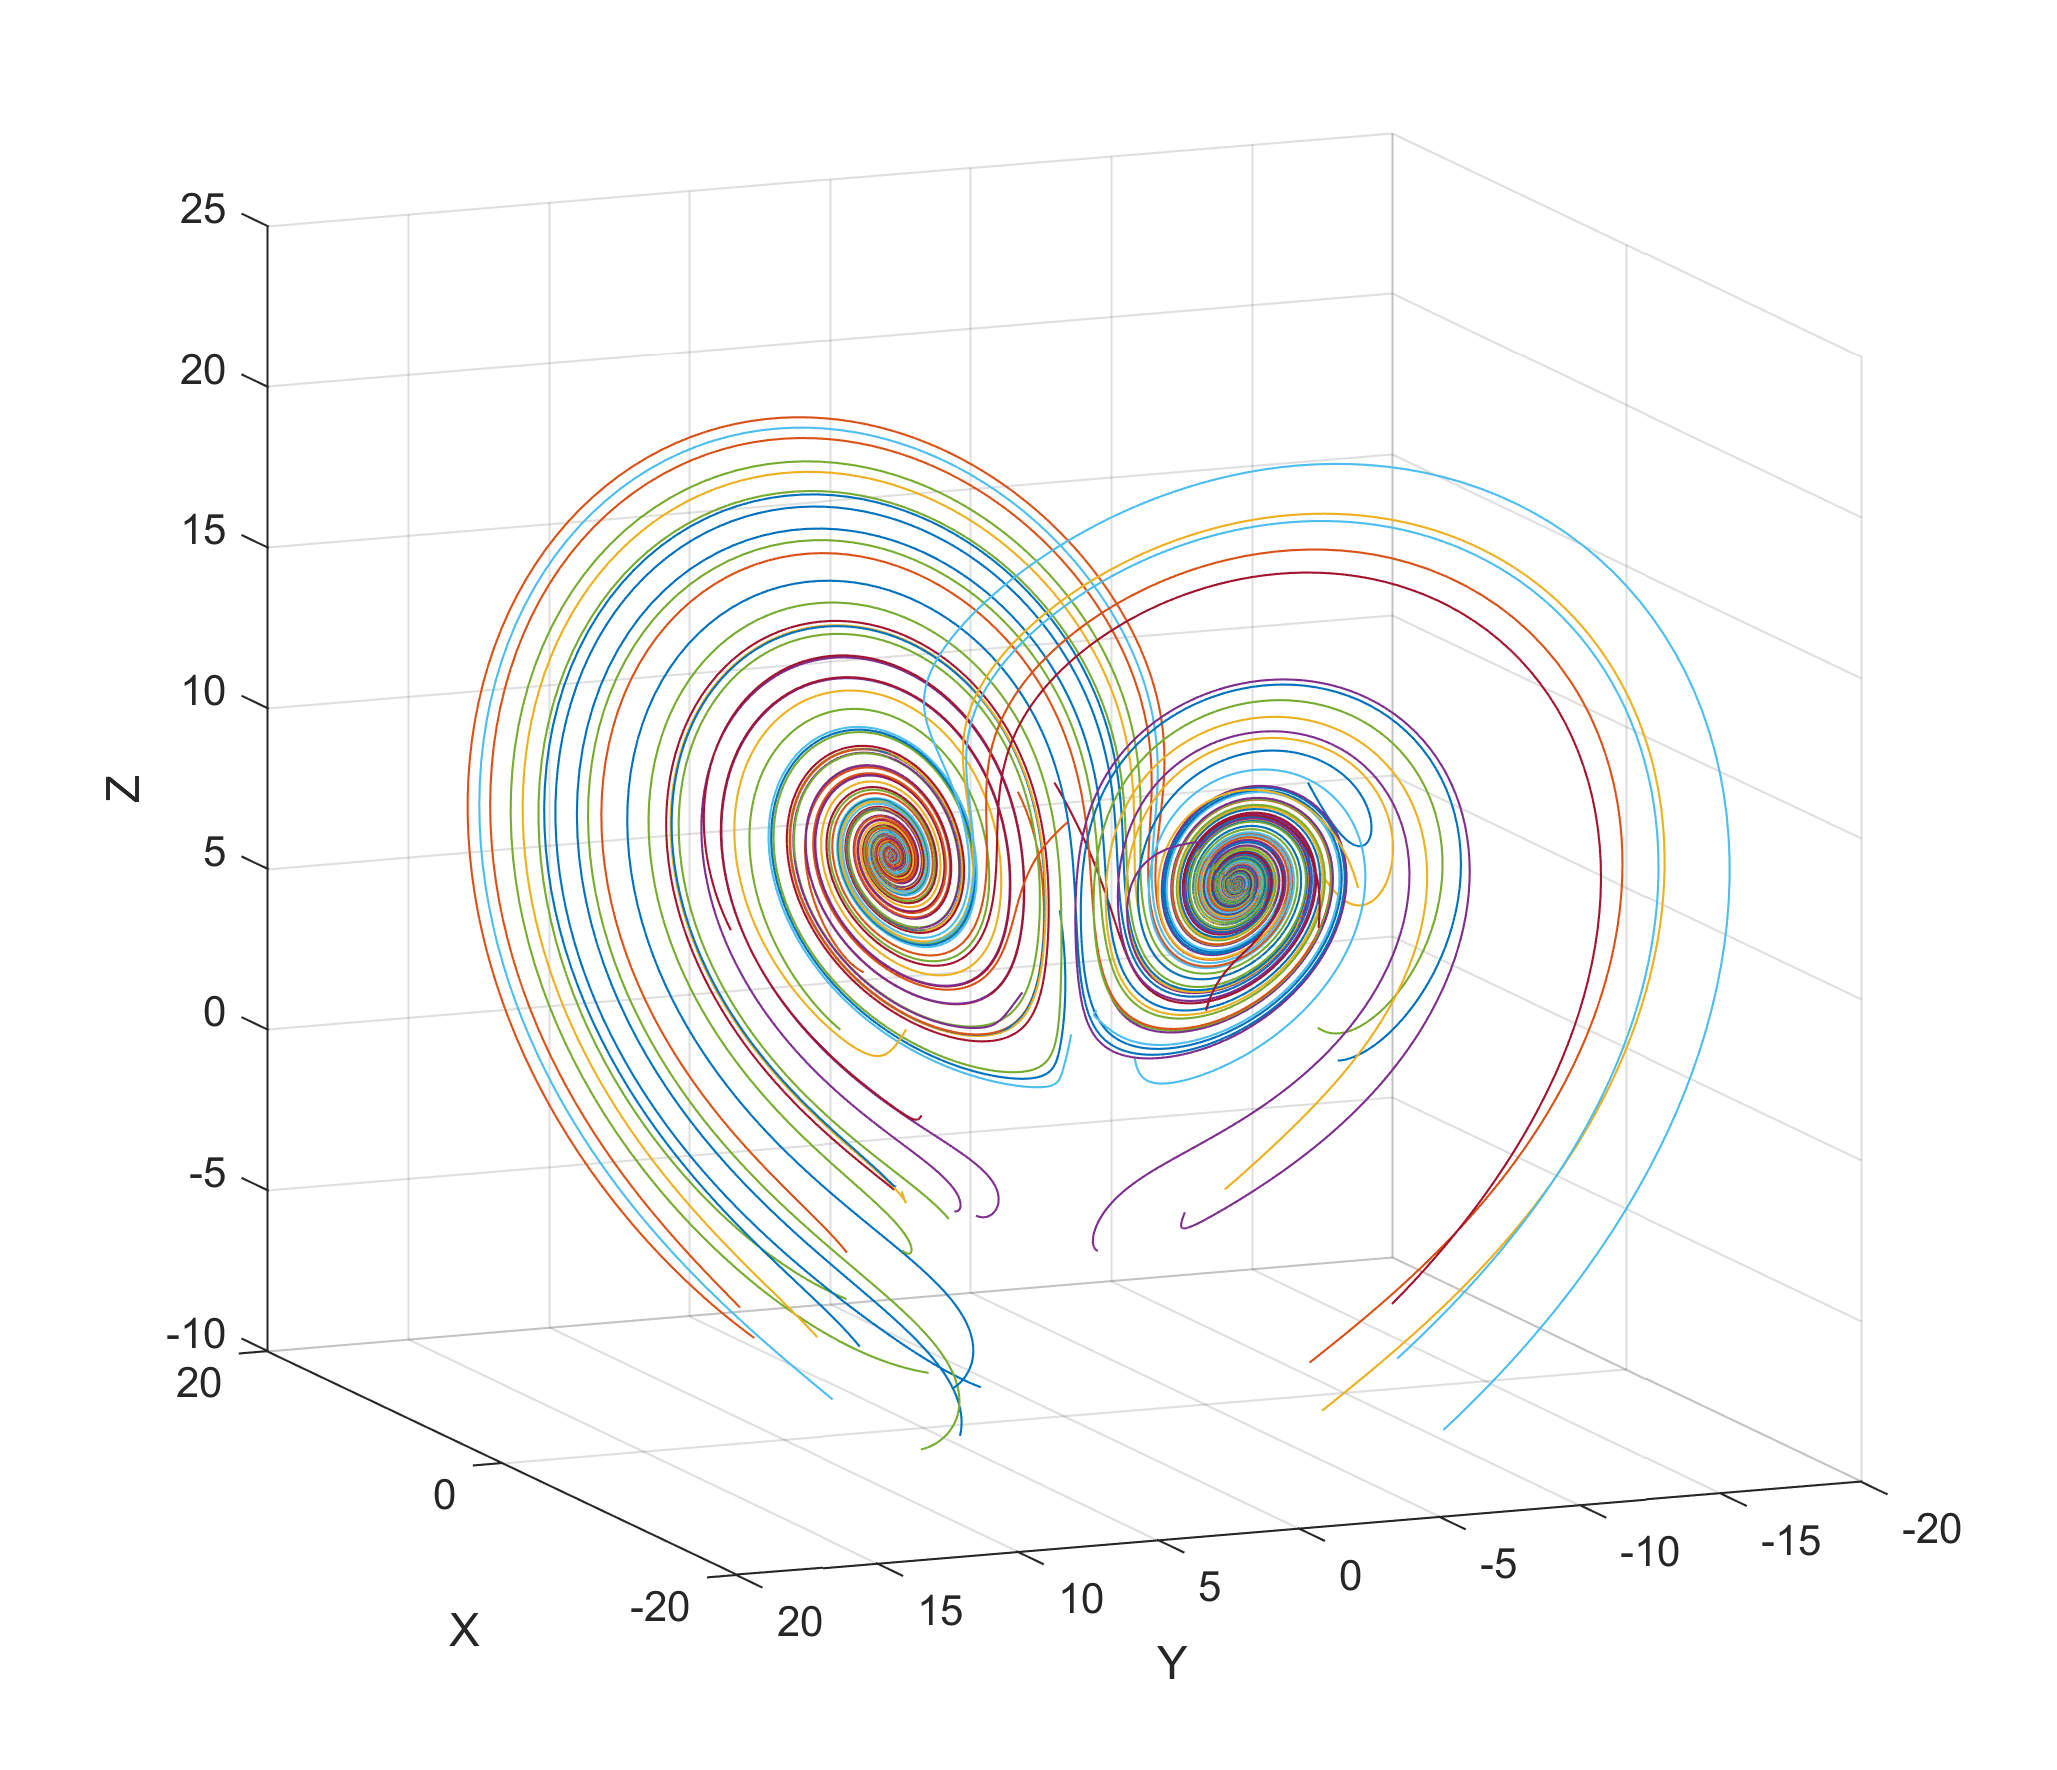
\includegraphics[width=8cm]{XYZ_r_8.png}  %需调整
        \caption{$r=8$,相空间轨迹}
    \end{minipage}
    \hfill %弹性长度
    \begin{minipage}[c]{0.45\linewidth}  %需调整
        \centering
        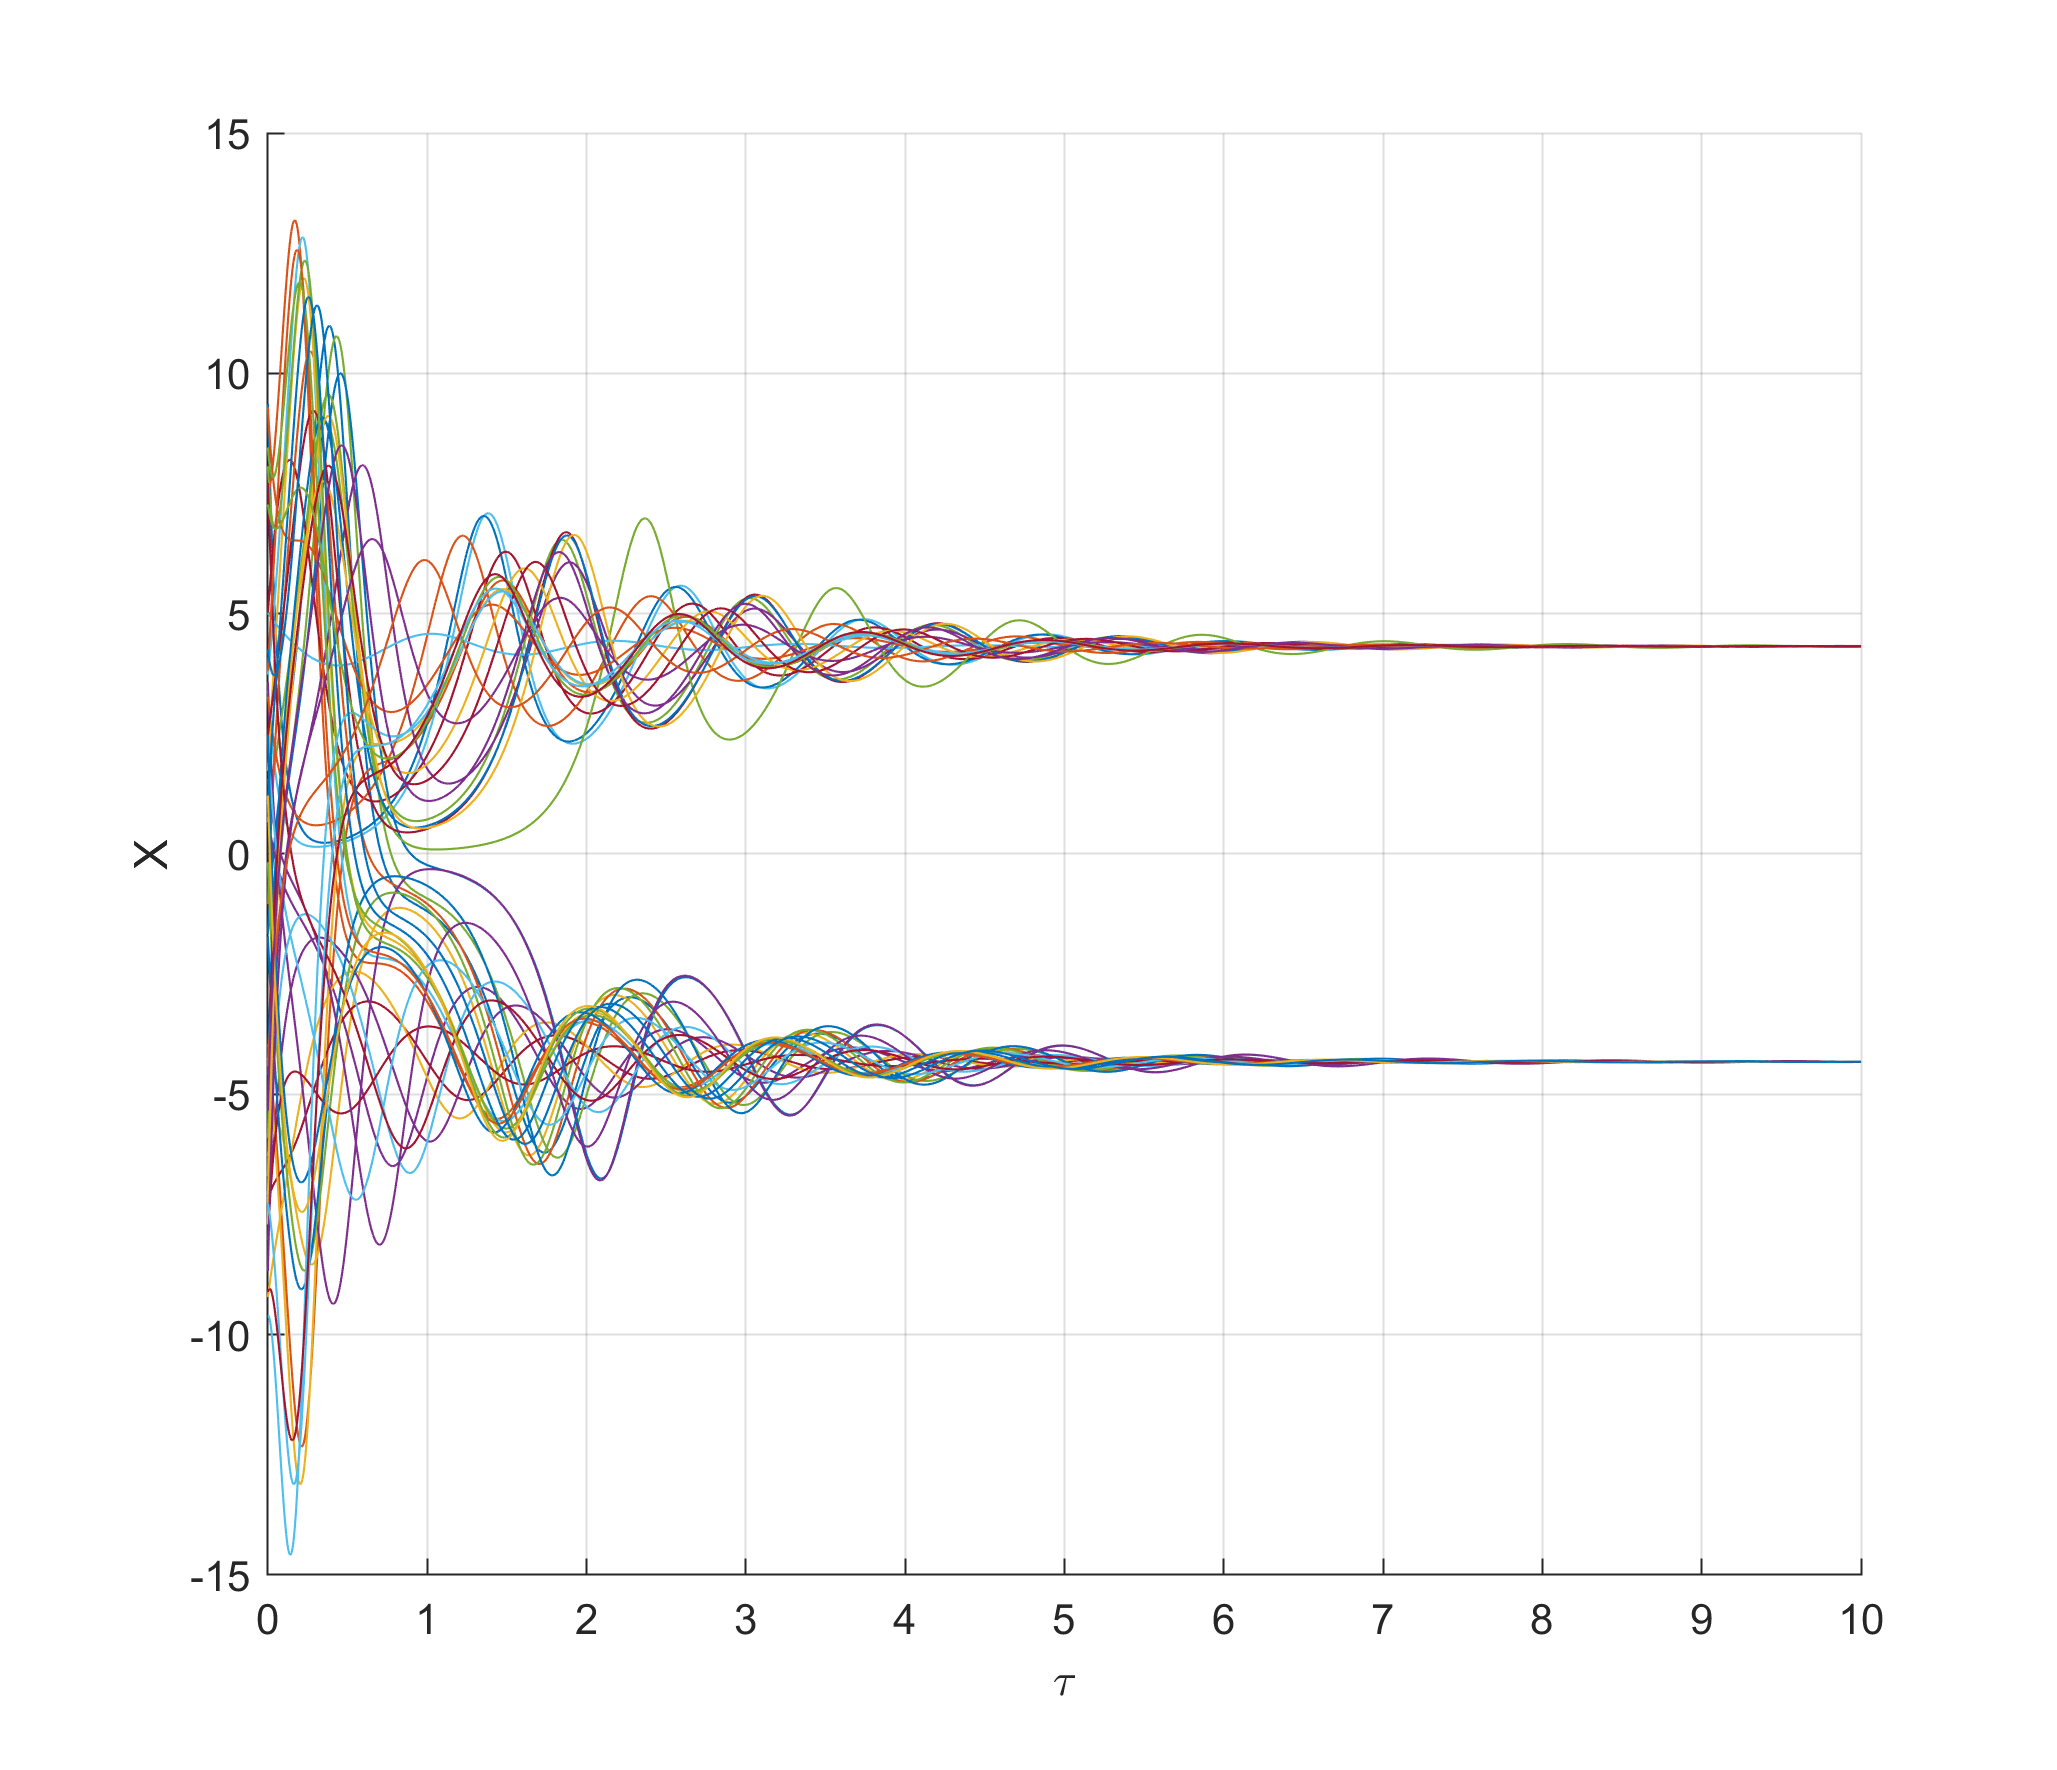
\includegraphics[width=8cm]{XT_r_8.png}  %需调整
        \caption{$r=8$,$X$沿时间变化}
    \end{minipage}
\end{figure}
可见此时0处的平衡点不稳定,但是新的两个非零平衡点是稳定的。根据线性分析,
可知$r<1.34$时是结点,大于时是焦点,图中可见当$r>1.34$,衰减过程变成强烈非单调的振荡过程。

\subsection{$13.926<r<24.06$}

选择$r=20$,不同初值计算,如下图
\begin{figure}[H]
    \begin{minipage}[c]{0.45\linewidth}  %需调整
        \centering
        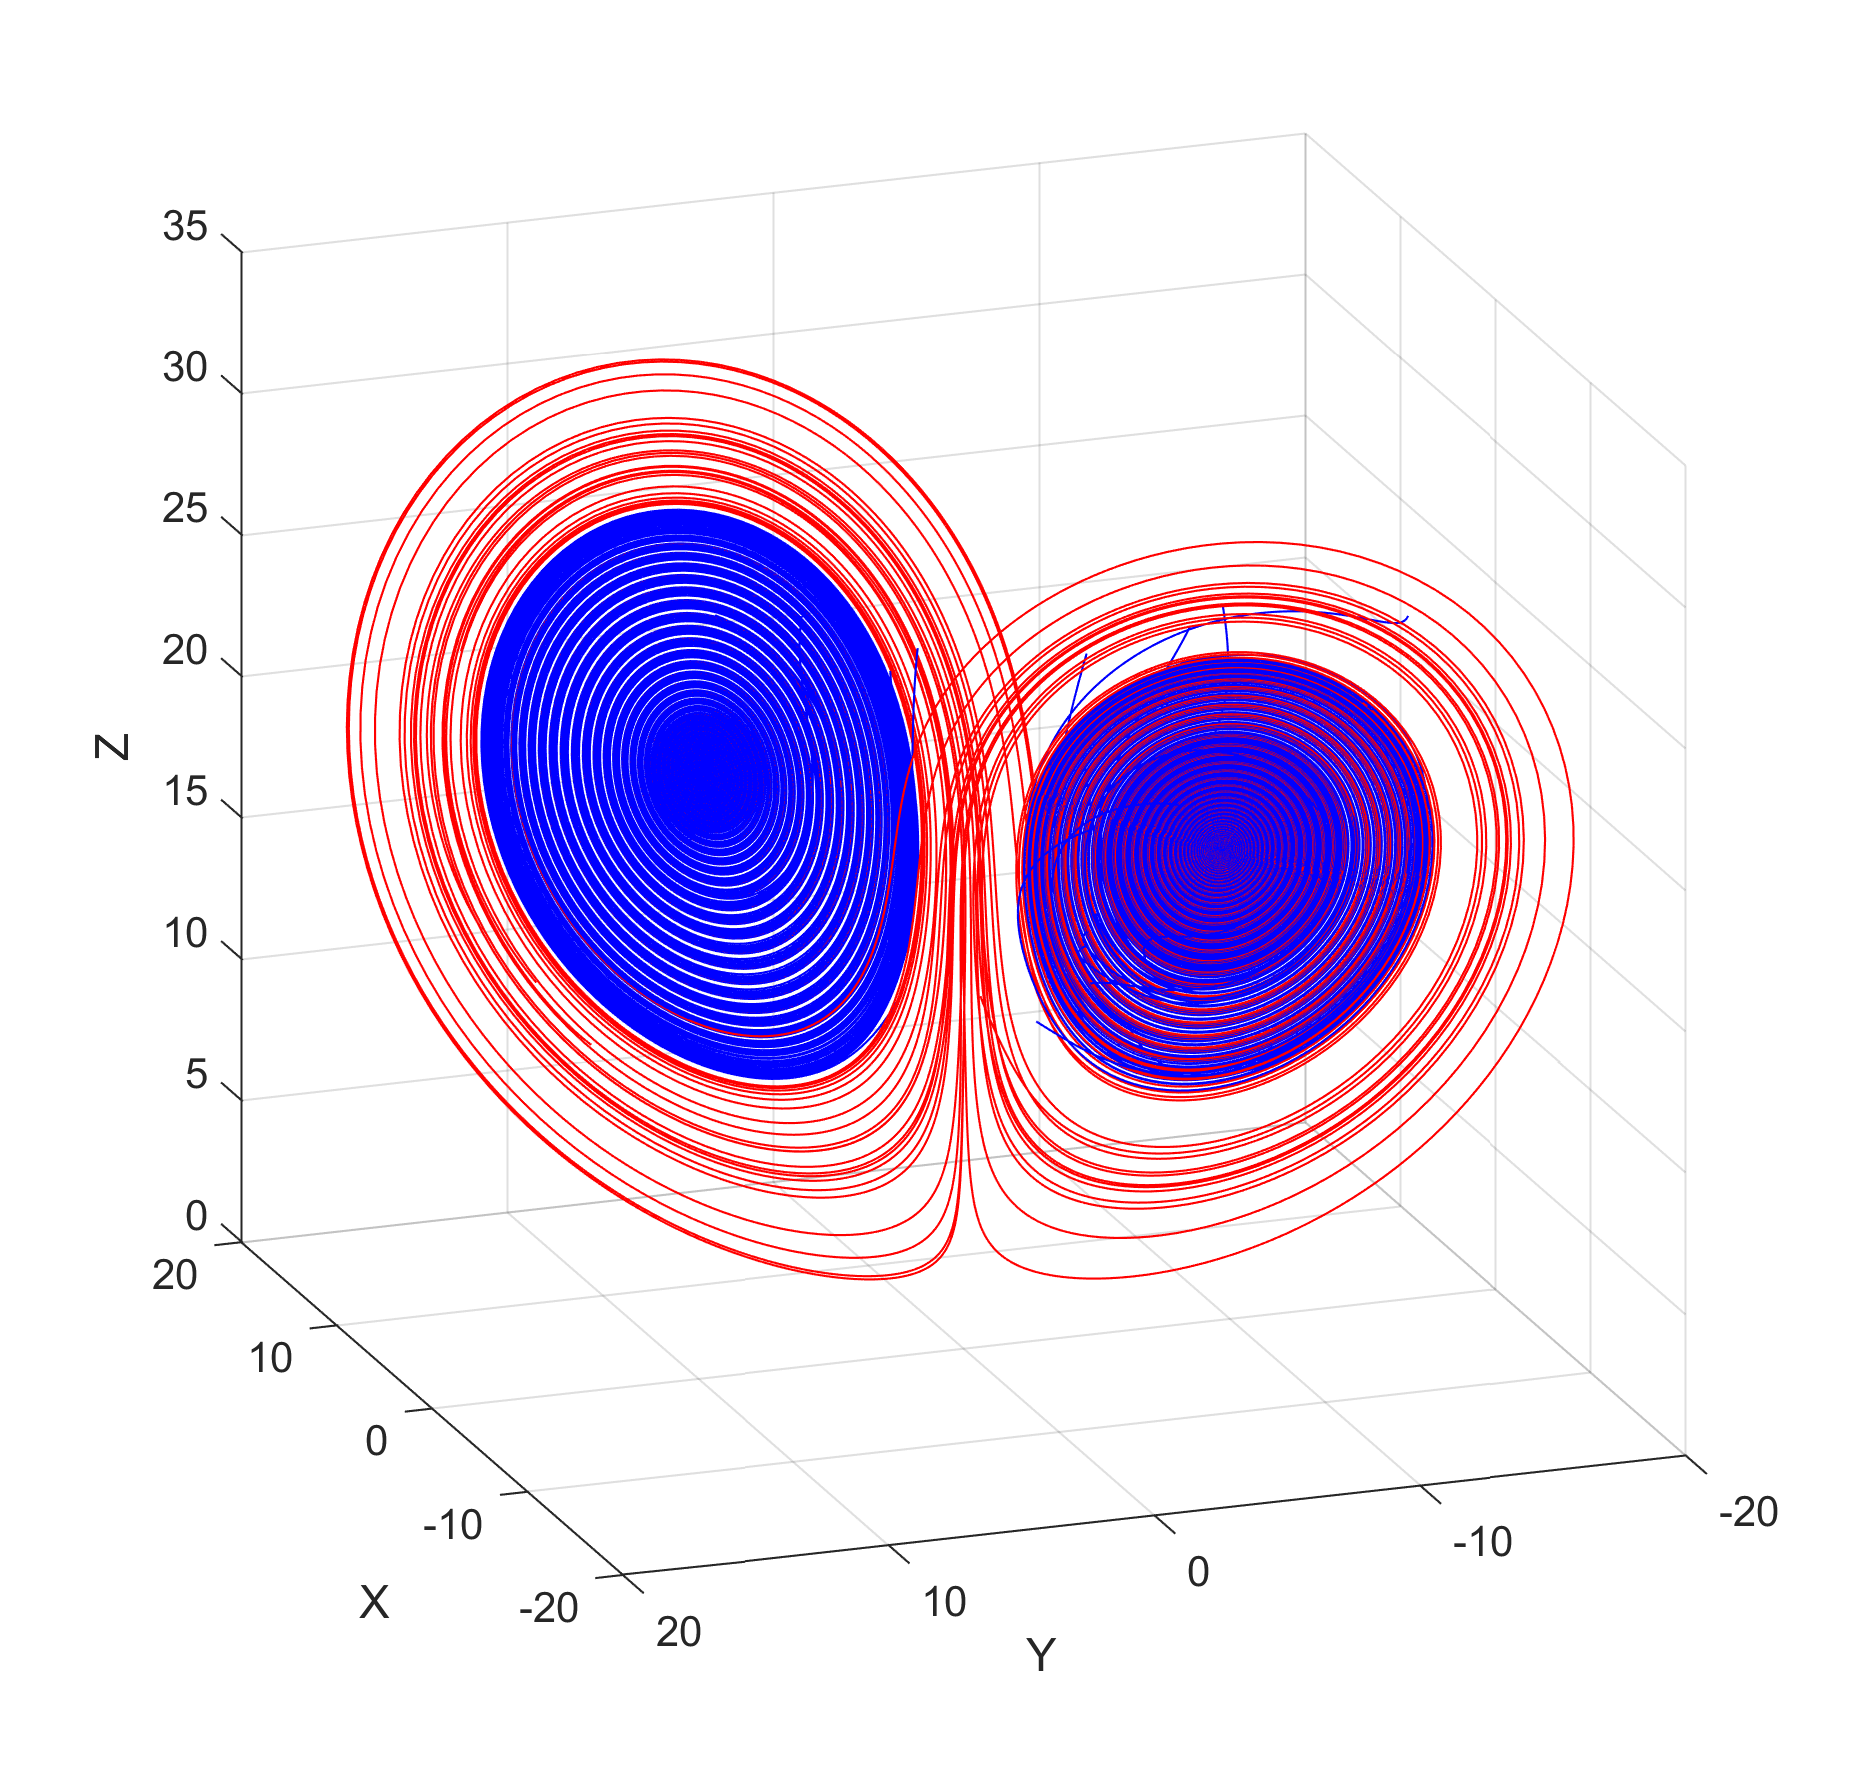
\includegraphics[width=8cm]{XYZ_r_20.png}  %需调整
        \caption{$r=20$,相空间轨迹}
    \end{minipage}
    \hfill %弹性长度
    \begin{minipage}[c]{0.45\linewidth}  %需调整
        \centering
        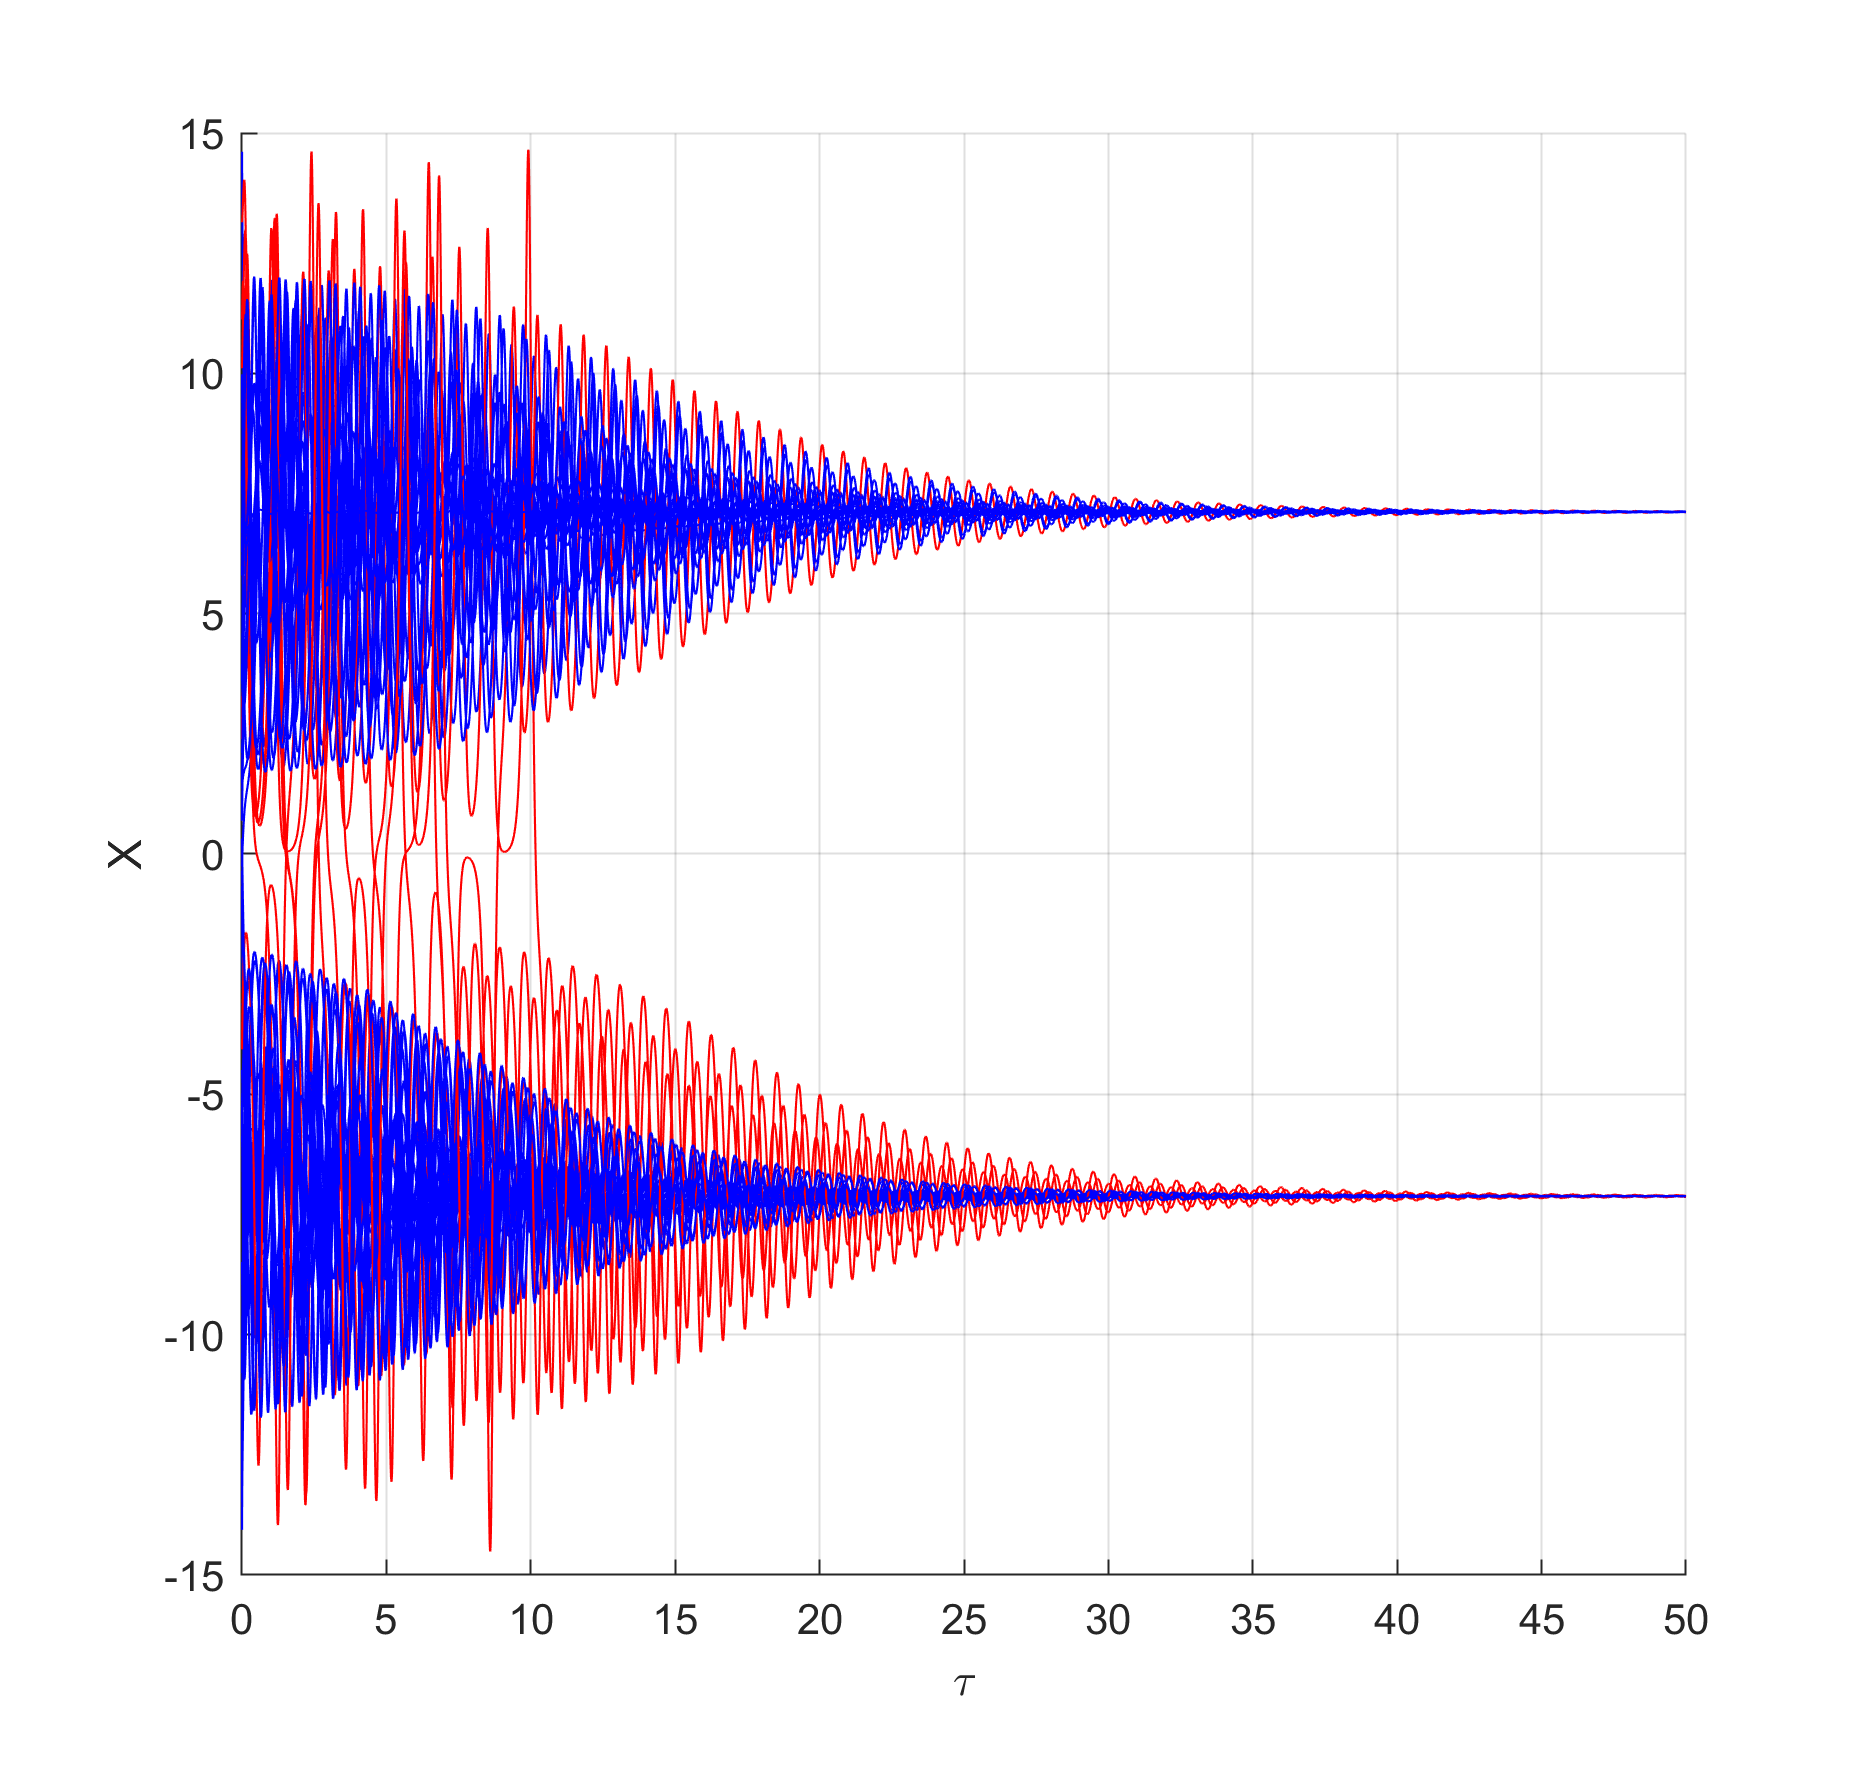
\includegraphics[width=8cm]{XT_r_20.png}  %需调整
        \caption{$r=20$,$X$沿时间变化}
    \end{minipage}
\end{figure}
图中从一个焦点跨越到另一个焦点的轨迹都画为红色。可见,此时焦点附近是线性稳定的,
但是焦点外侧有一个不稳定的极限环,极限环外侧振幅增大,内侧振幅减小。此时,
极限环外侧的轨迹构成短暂的混沌现象。

\subsection{$24.06<r<24.74$}

选择$r=24.1$,不同初值计算,如下图
\begin{figure}[H]
    \begin{minipage}[c]{0.45\linewidth}  %需调整
        \centering
        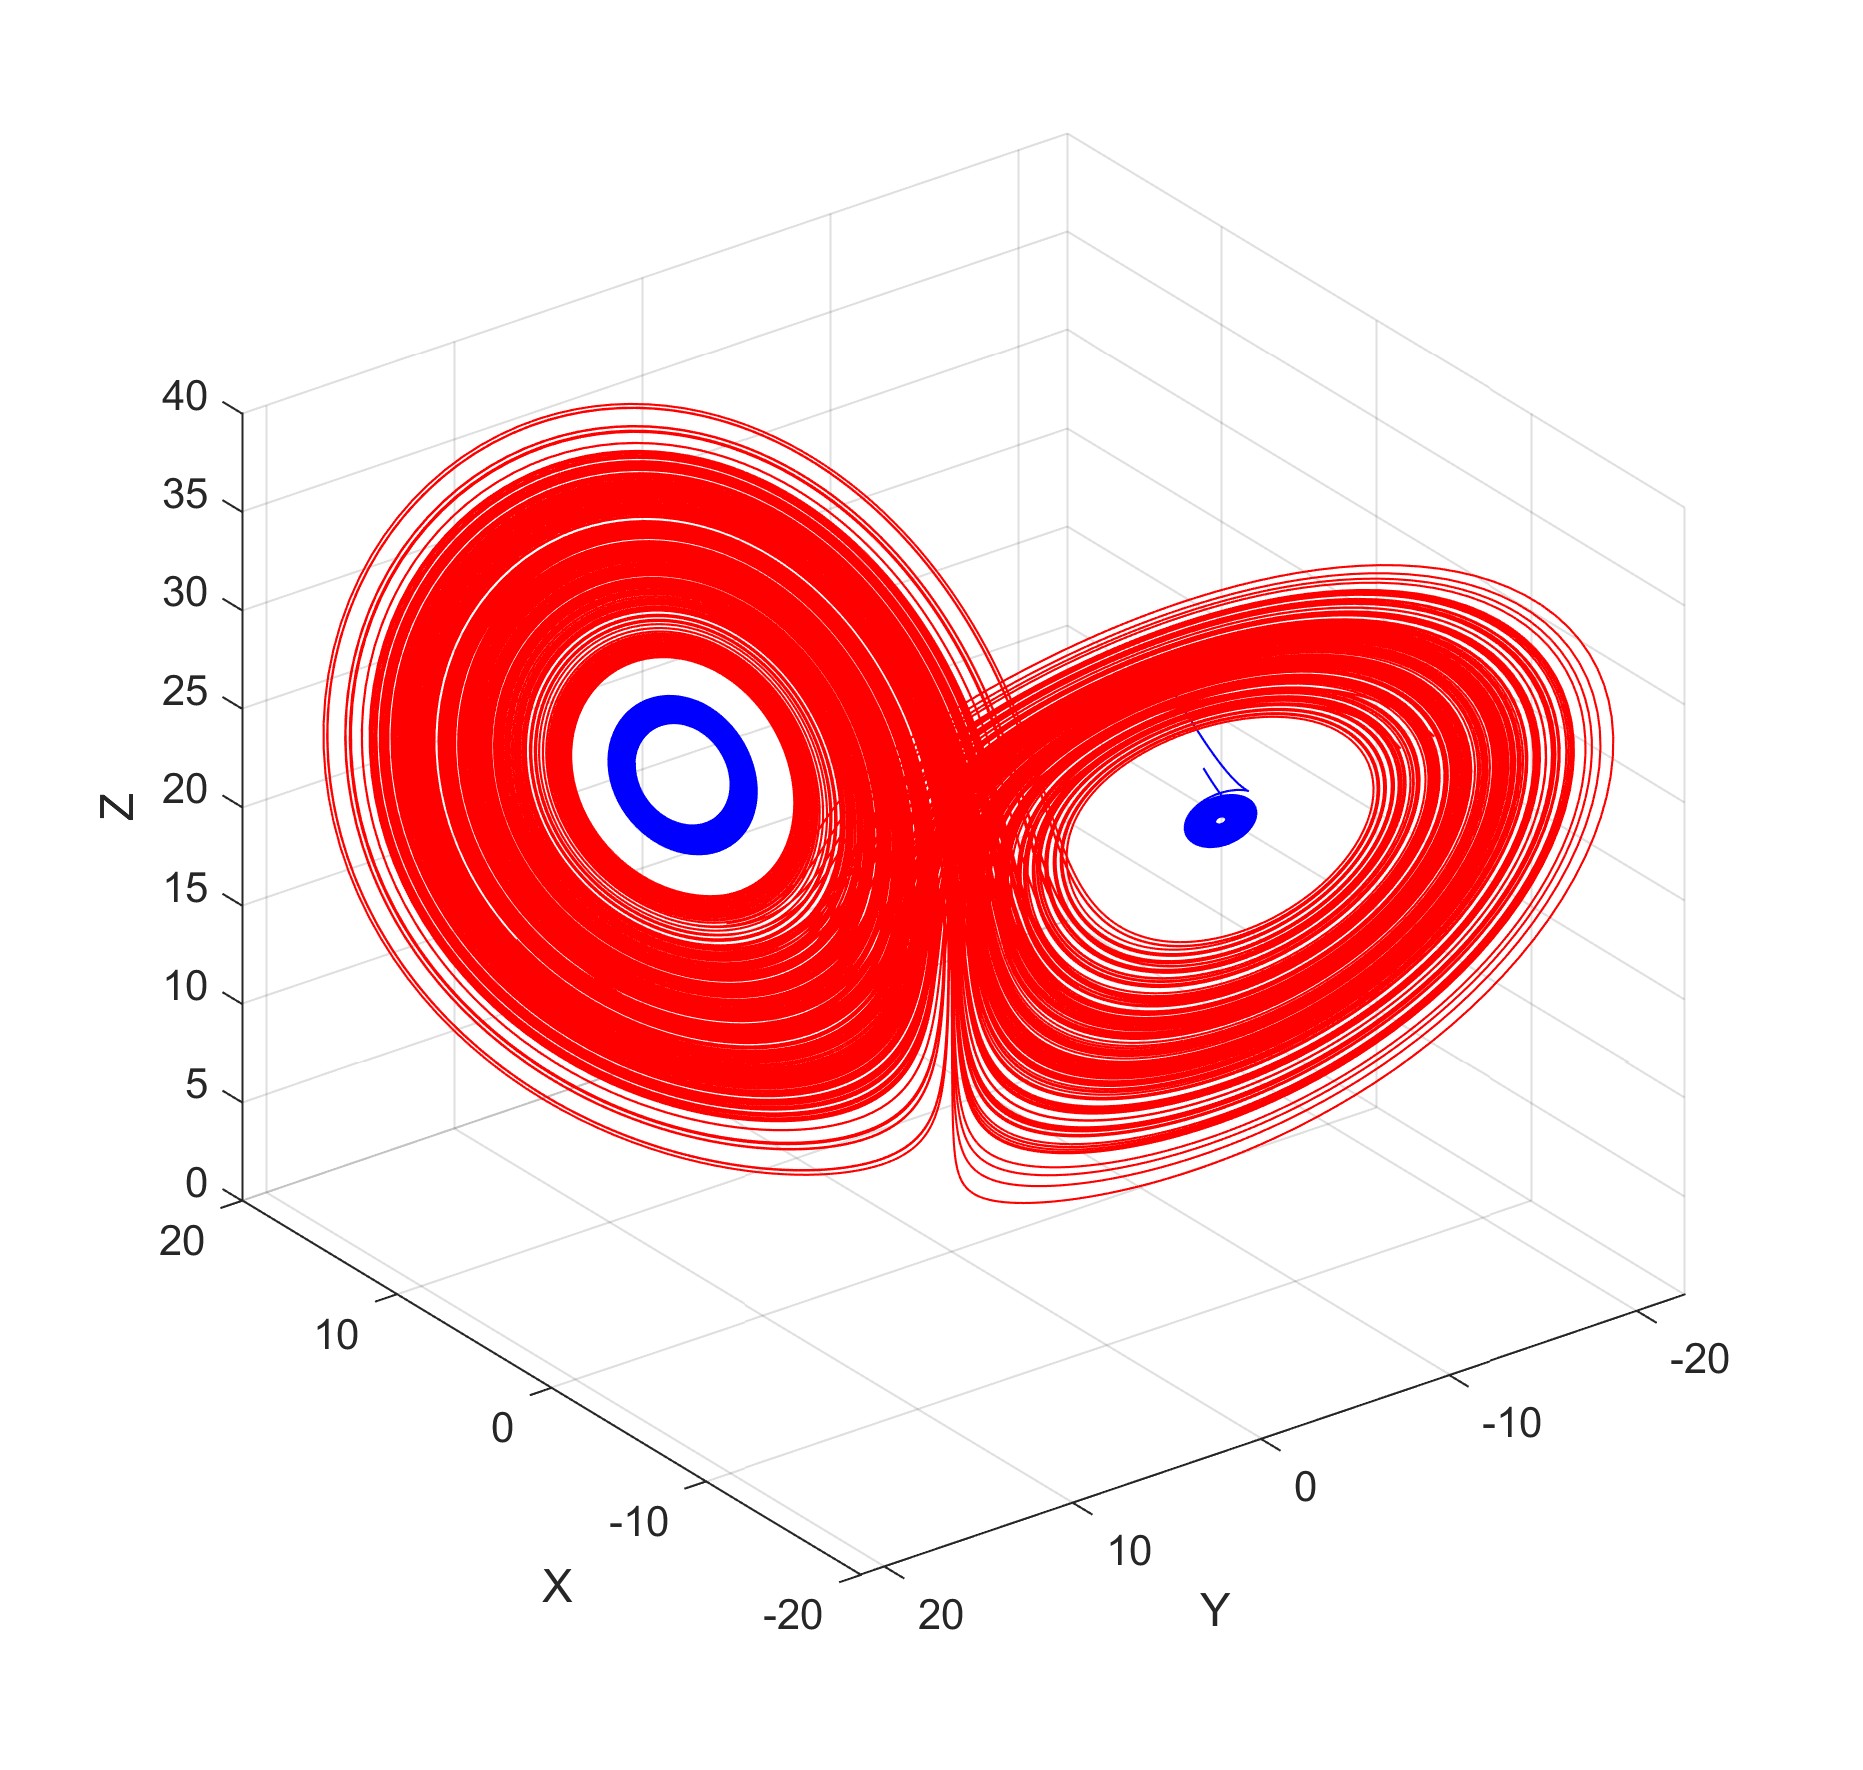
\includegraphics[width=8cm]{XYZ_r_24.1.png}  %需调整
        \caption{$r=24.1$,相空间轨迹}
    \end{minipage}
    \hfill %弹性长度
    \begin{minipage}[c]{0.45\linewidth}  %需调整
        \centering
        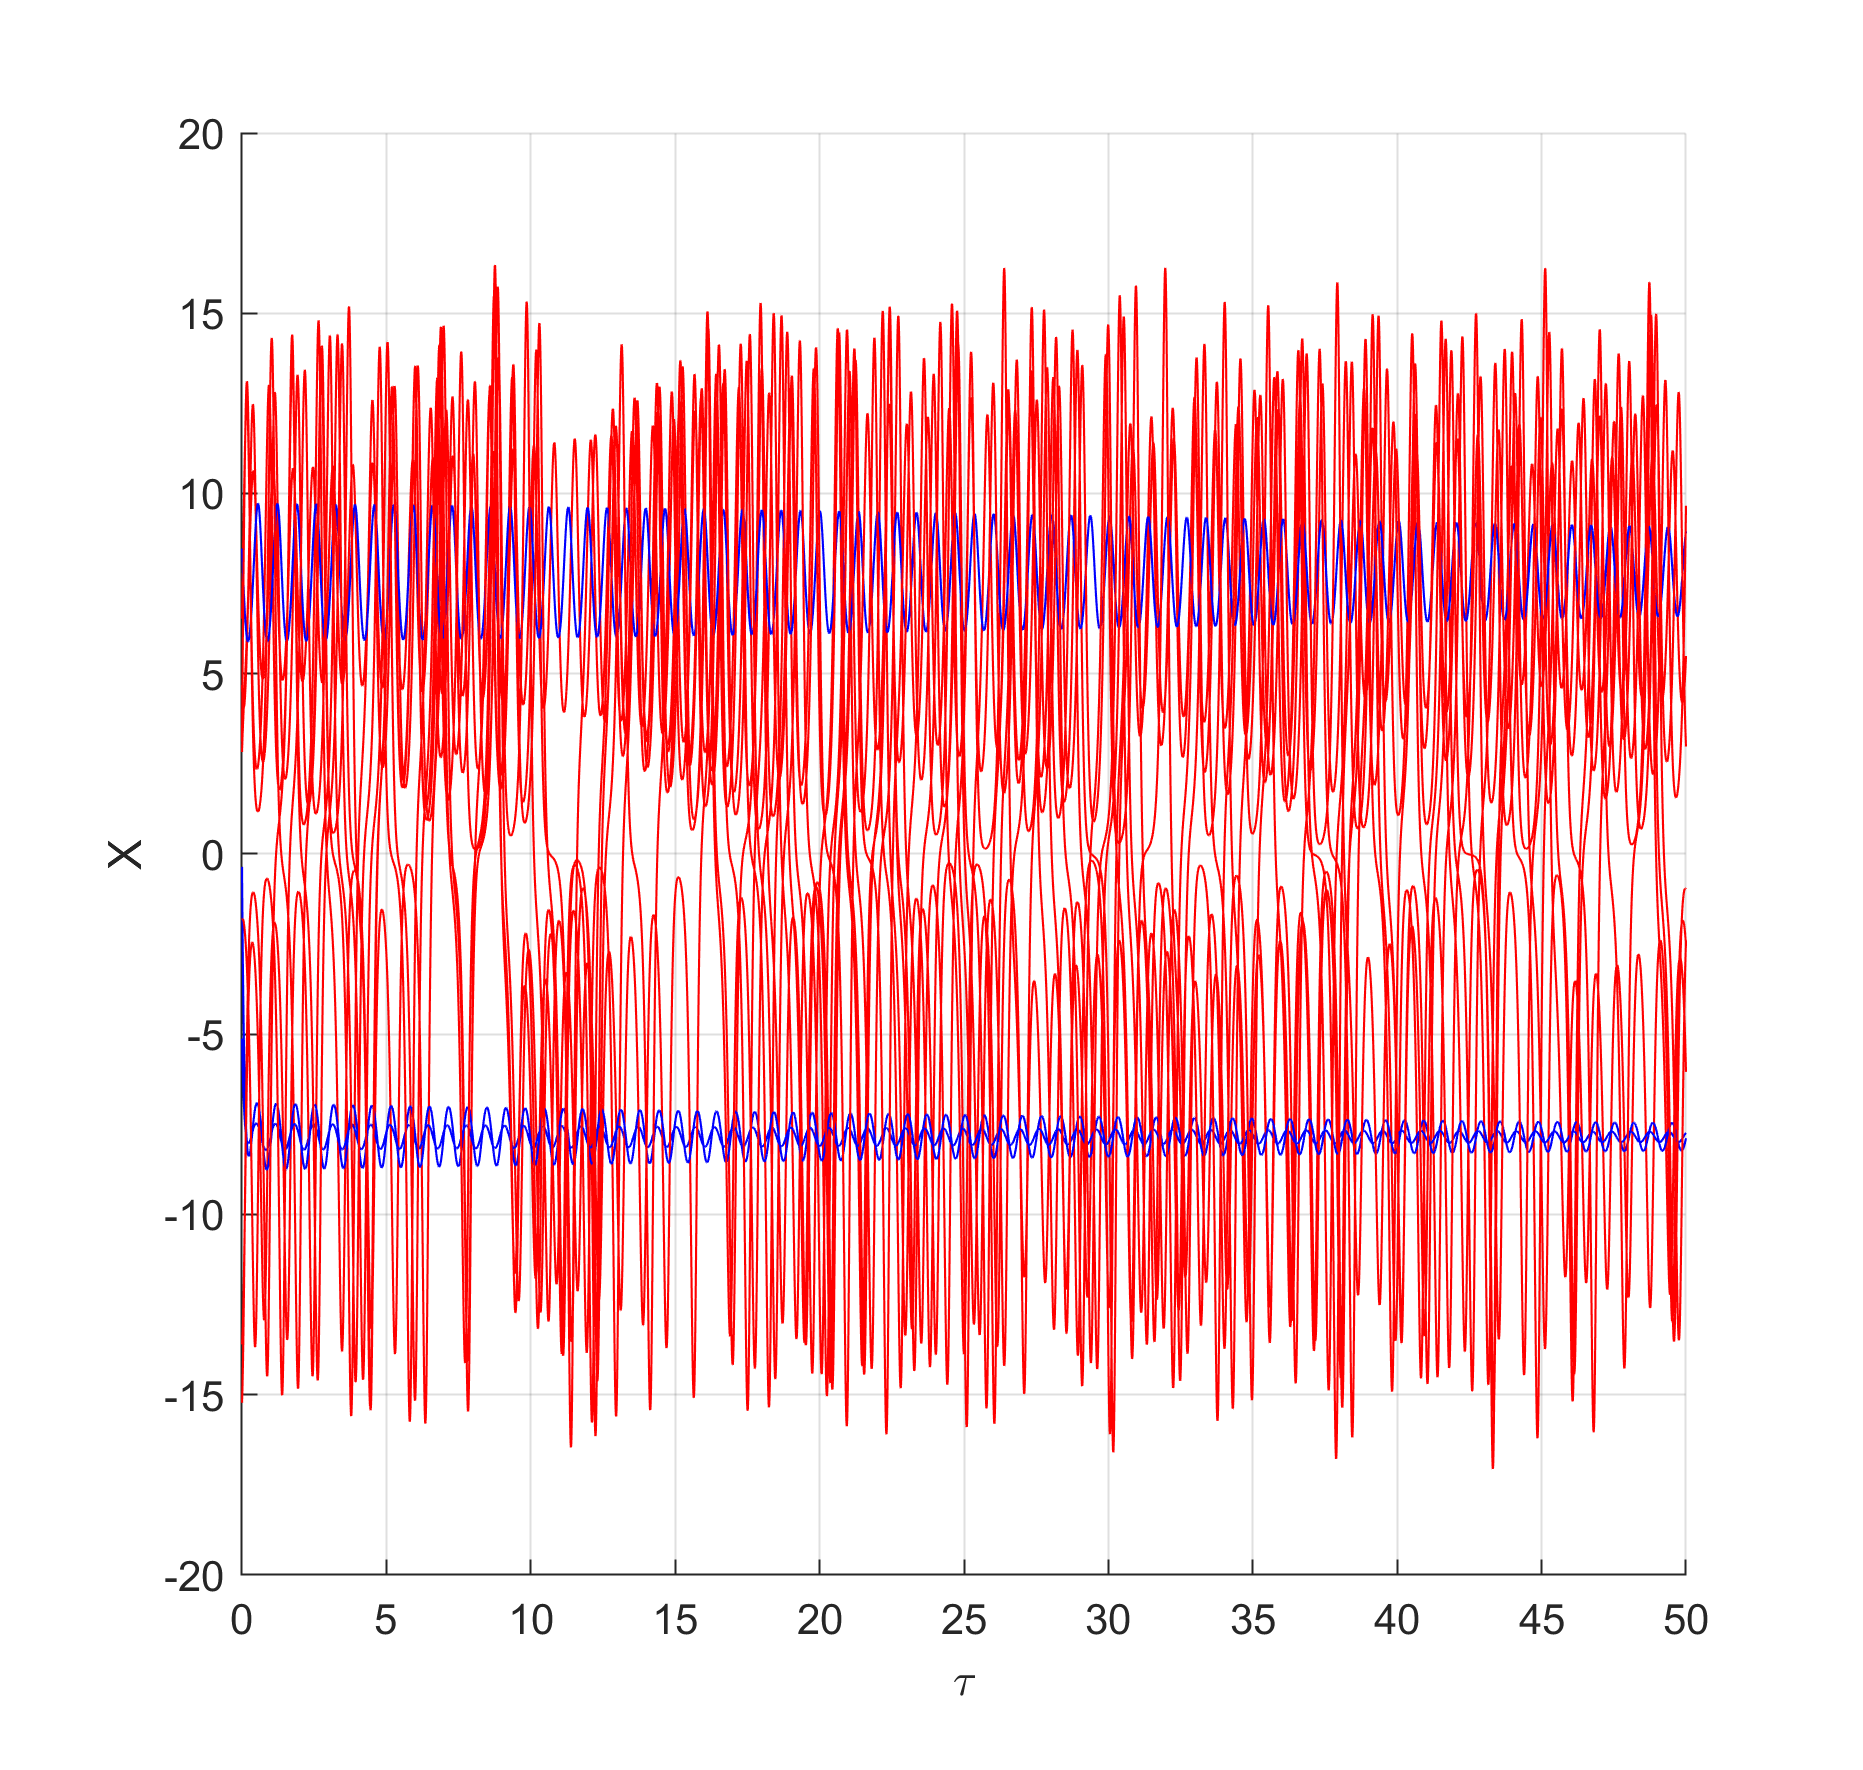
\includegraphics[width=8cm]{XT_r_24.1.png}  %需调整
        \caption{$r=24.1$,$X$沿时间变化}
    \end{minipage}
\end{figure}
图中从一个焦点跨越到另一个焦点的轨迹都画为红色。此时焦点附近是线性稳定的,
但是一旦落到极限环之外,就处于持续的混沌中,只有极限环内部的轨迹能衰减。

\subsection{$24.74<r$}

选择$r=25$,不同初值计算,如下图
\begin{figure}[H]
    \begin{minipage}[c]{0.45\linewidth}  %需调整
        \centering
        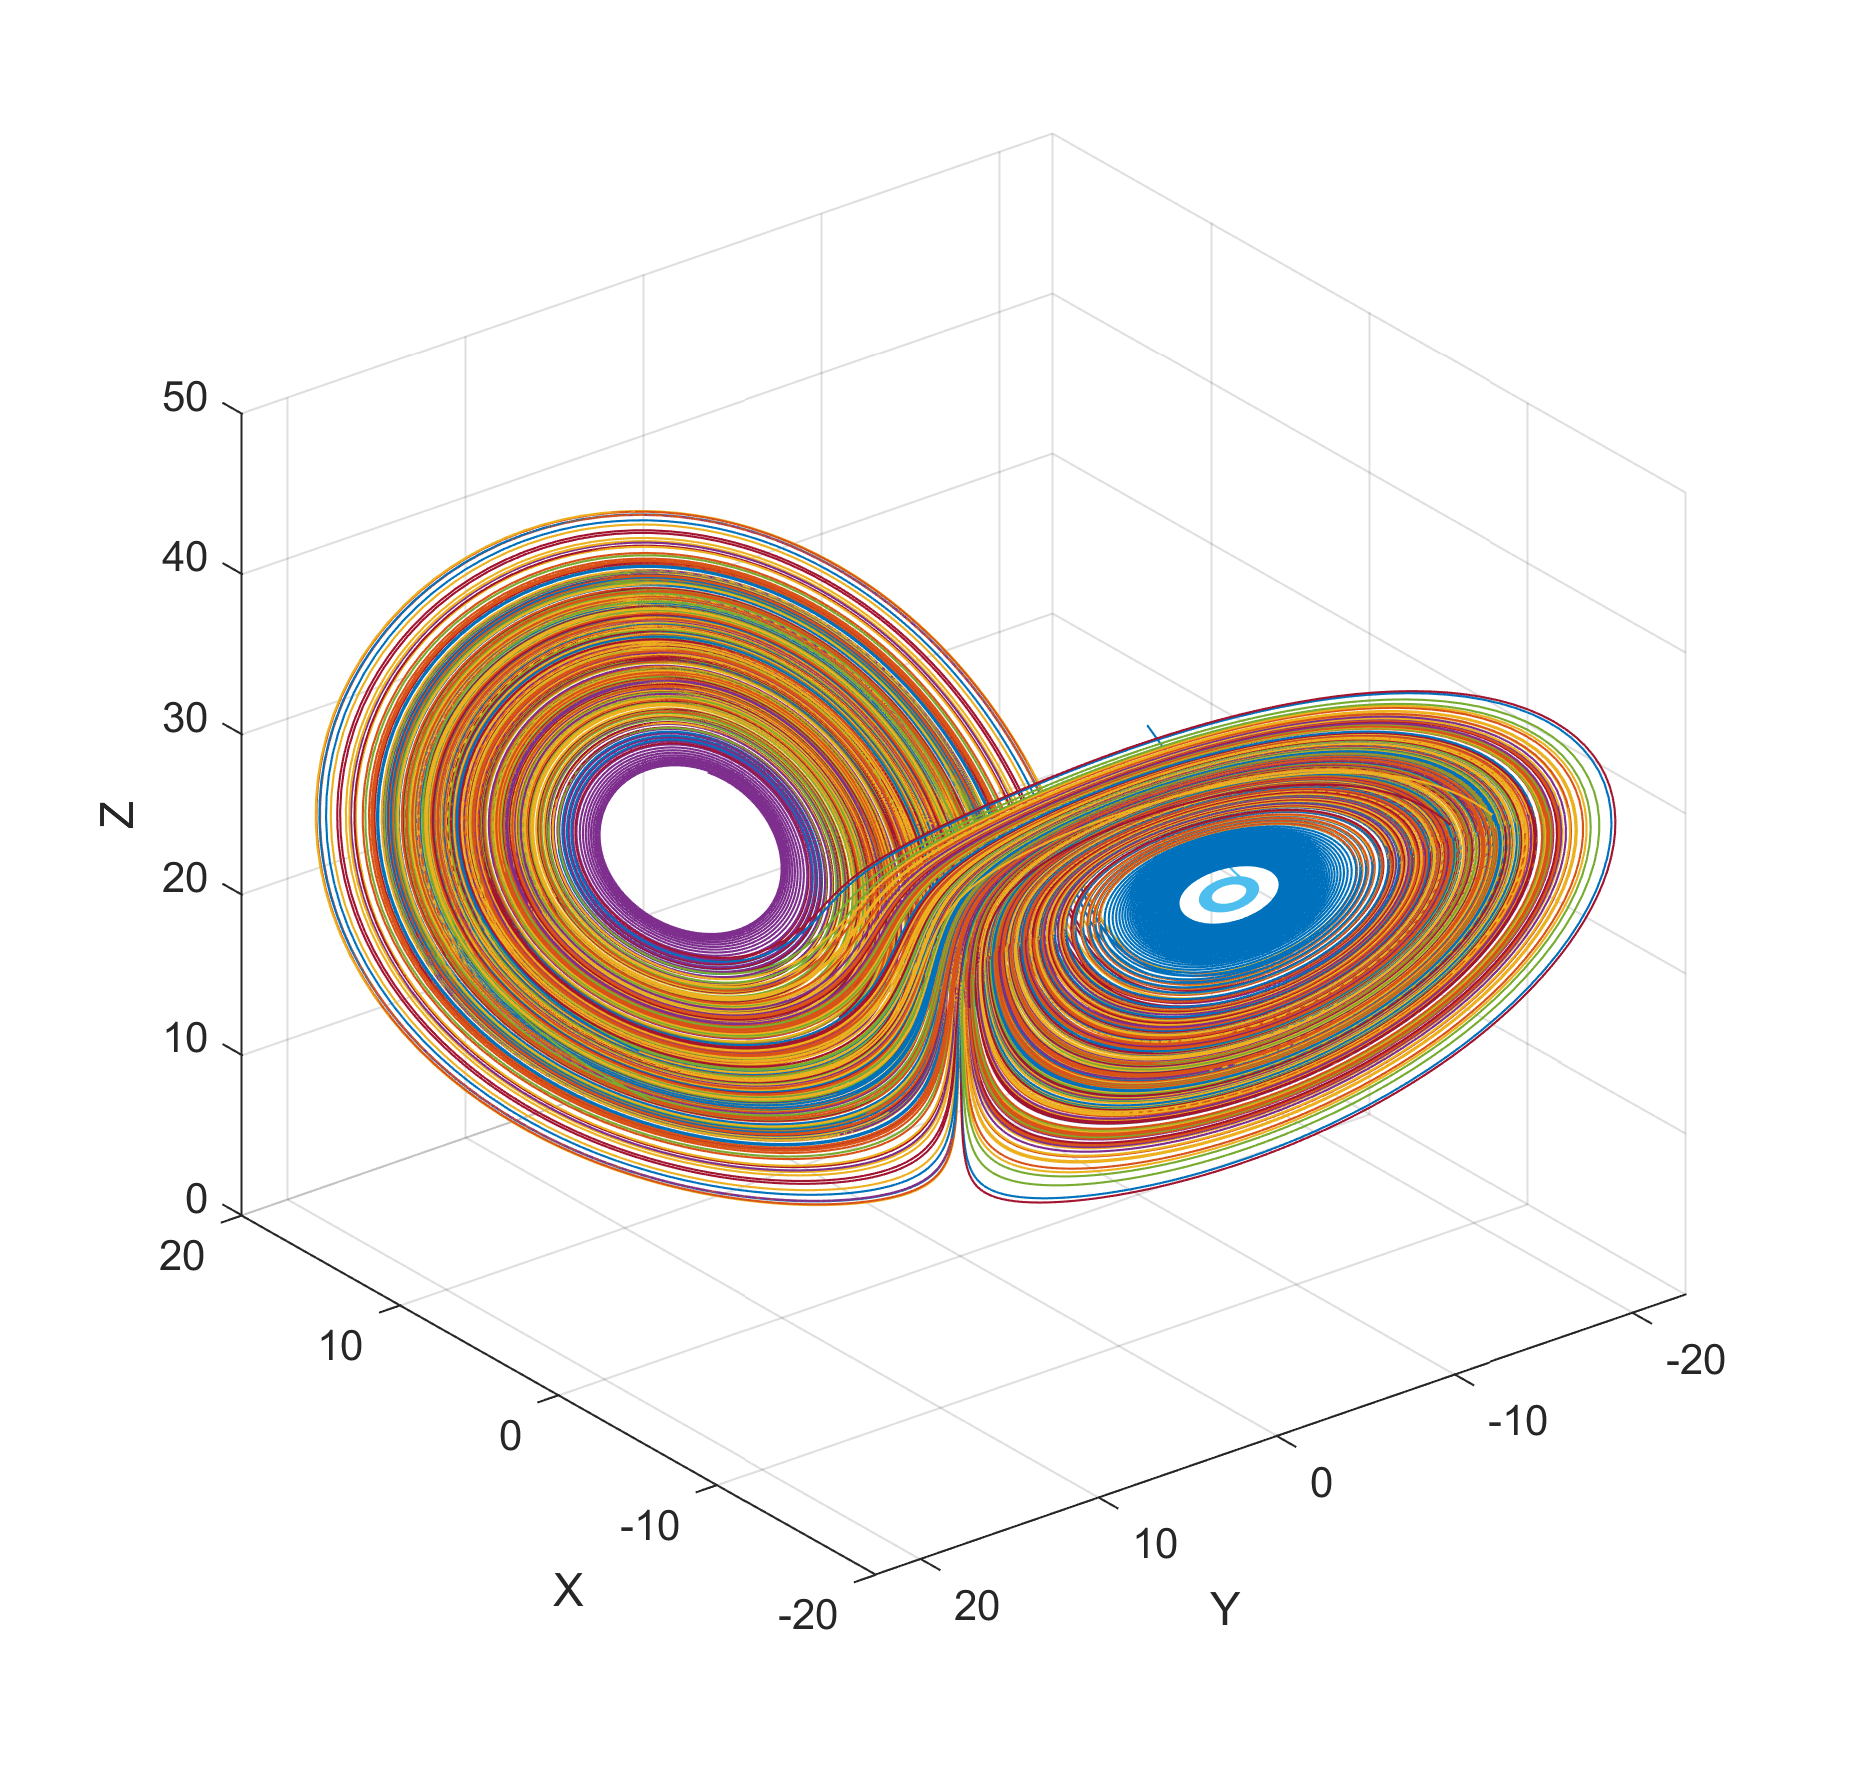
\includegraphics[width=8cm]{XYZ_r_25.png}  %需调整
        \caption{$r=25$,相空间轨迹}
    \end{minipage}
    \hfill %弹性长度
    \begin{minipage}[c]{0.45\linewidth}  %需调整
        \centering
        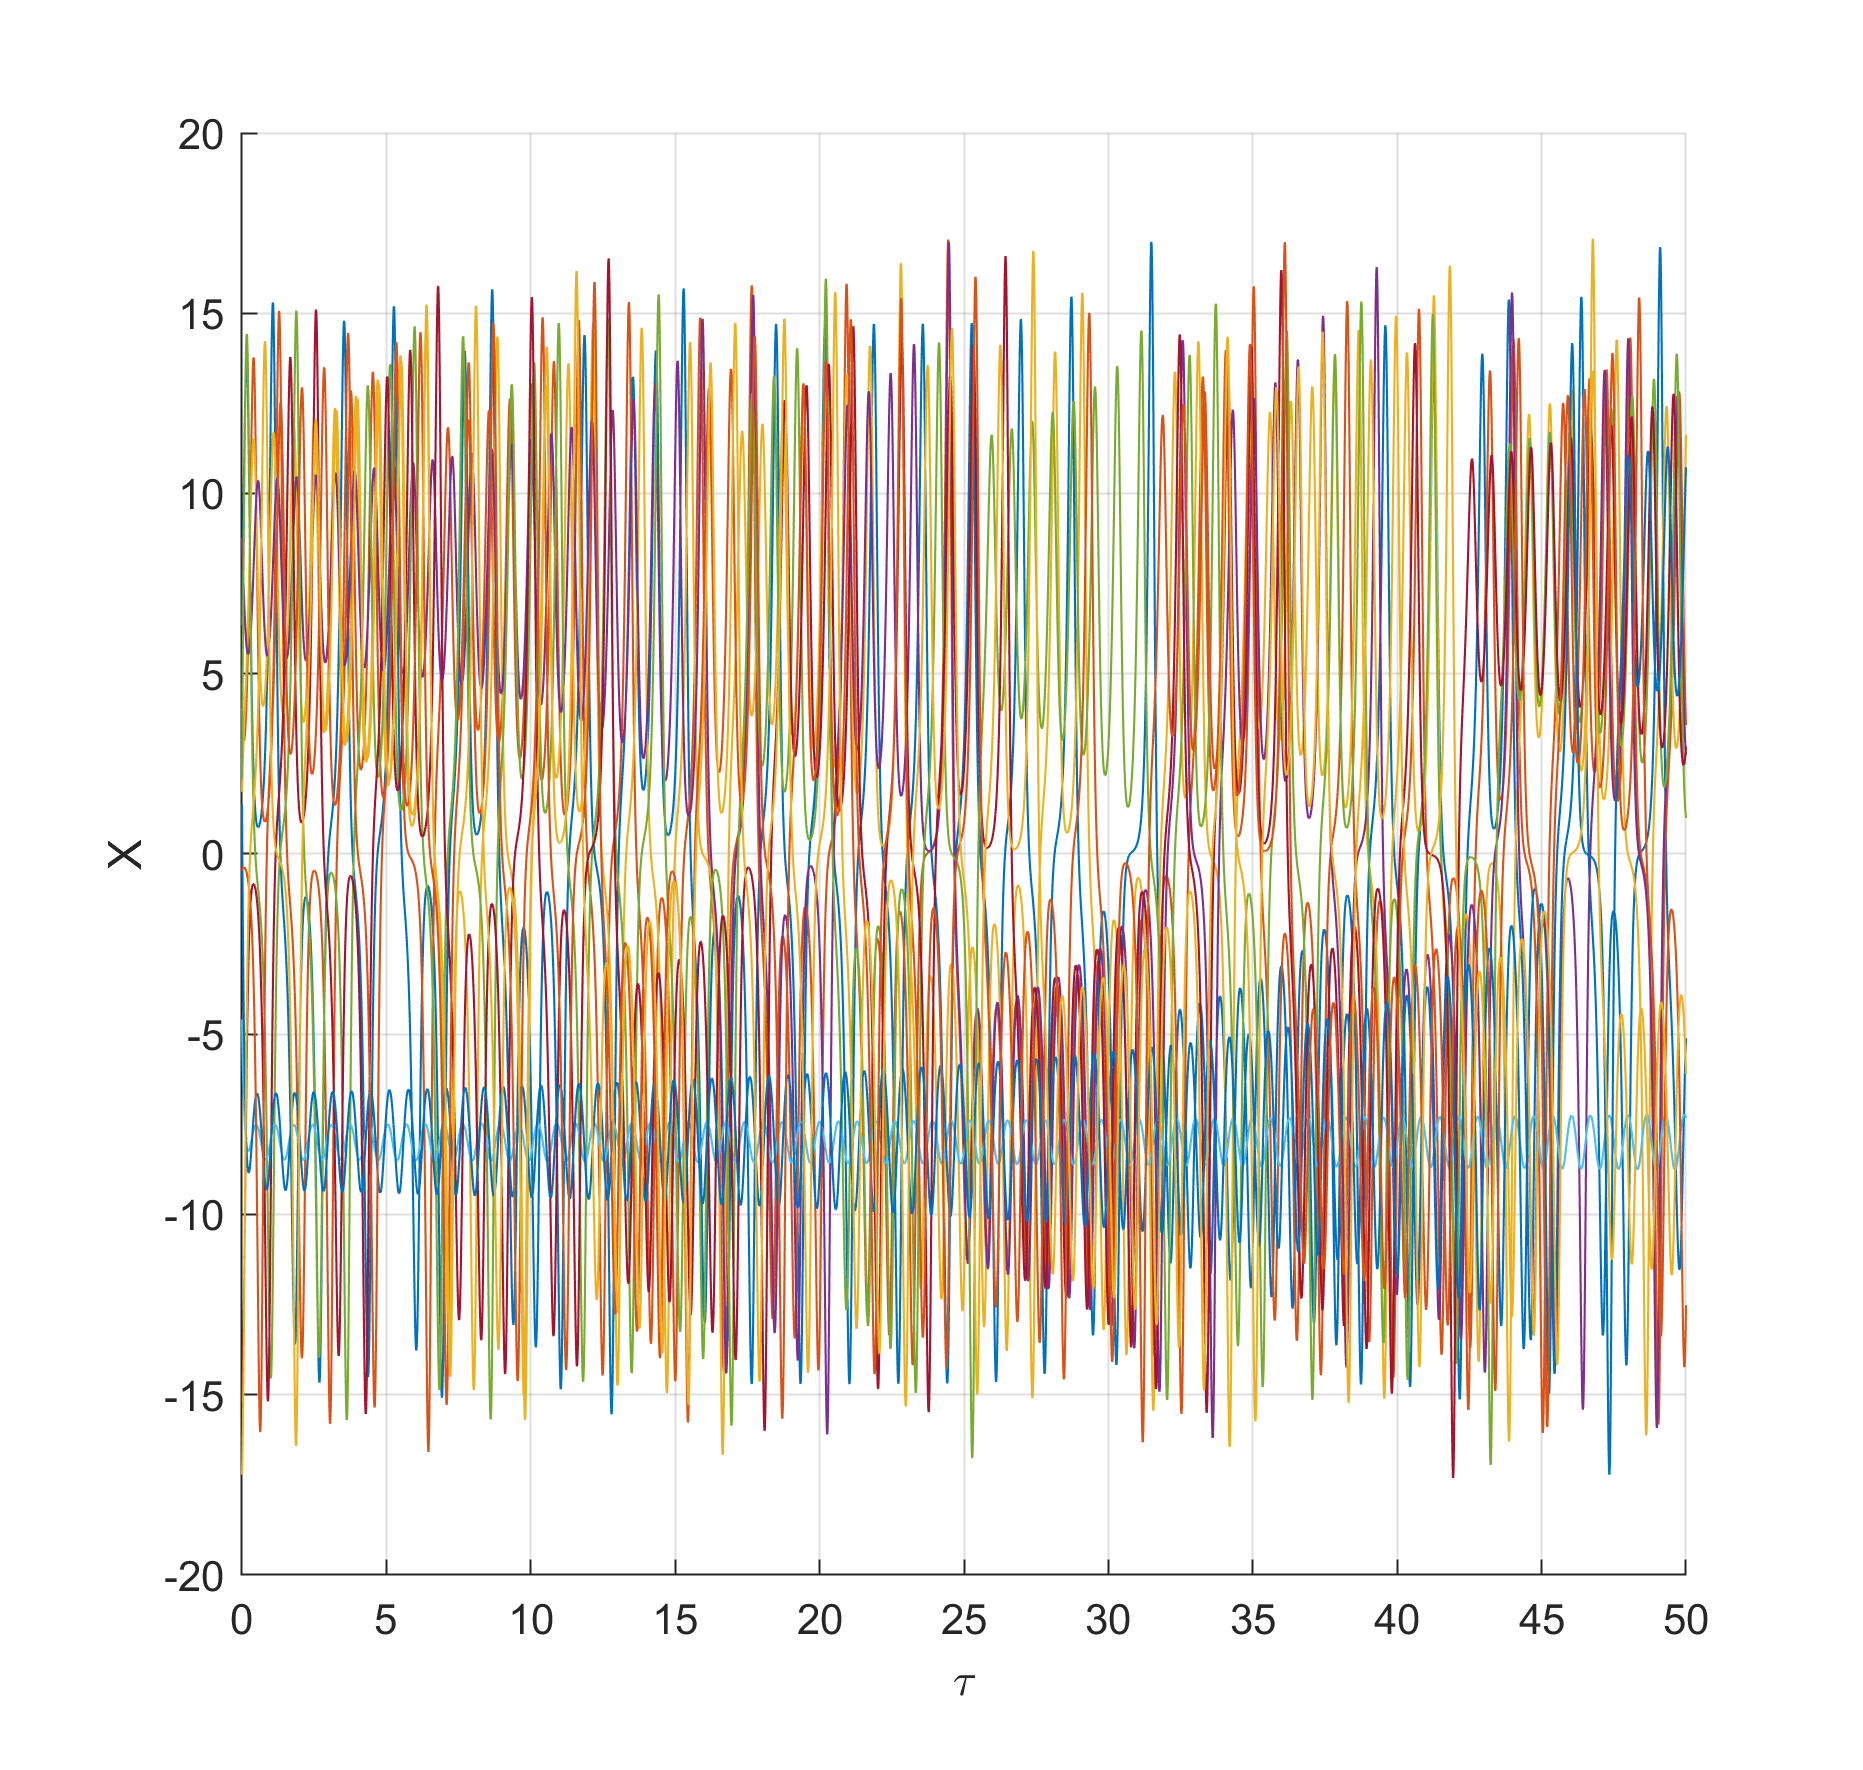
\includegraphics[width=8cm]{XT_r_25.png}  %需调整
        \caption{$r=25$,$X$沿时间变化}
    \end{minipage}
\end{figure}
此时焦点附近线性不稳定,所有轨迹都处于混沌状态。

\section{附录}
本文计算代码都在\href{https://github.com/harryzhou2000/HW_ACFD}{Github Repo中(点击访问)}。































% \section{SECTION 节}

% 一个

% \subsection{SUBSECTION 小节}

% 示例

% \subsubsection{SUBSUBSECTION 小节节}

% 字体字号临时调整:
% {
%    \sffamily\bfseries\zihao{3} 哈哈哈哈哈 abcde %三号 sans系列字体(一开始设置的) 加粗
%    %只对大括号范围内的后面的字有用,在标题、题注里面同样
% }
% { 
%    \CJKfamily{kaiti}\zihao{5}\itshape 哈哈哈哈哈 abcde%三号 kaiti(一开始设置的, 斜体(英文有变)
%    %只对大括号范围内的后面的字有用,在标题、题注里面同样
% }

% 一大堆一大堆一大堆一大堆一大堆一大堆一大堆一大堆一大堆一大堆
% 一大堆一大堆一大堆一大堆一大堆一大堆一大堆一大堆一大堆一大堆一大堆一大堆
% 一大堆一大堆一大堆一大堆一大堆一大堆一大堆一大堆一大堆一大堆一大堆一大堆
% 一大堆一大堆一大堆一大堆一大堆一大堆一大堆一大堆一大堆一大堆一大堆一大堆

% \begin{center}
%     居中的什么乱七八糟东西
% \end{center}


% 一个列表:
% \begin{itemize}
%     \item asef
%     \item[\%] asdf
%     \item[\#] aaa
% \end{itemize}

% 一个有序列表:
% \begin{enumerate}
%     \item asef
%     \item[\%\%] asdf
%     \item aaa
% \end{enumerate}

% 一个嵌套列表,考虑缩进:
% \begin{enumerate}[itemindent=2em] %缩进
%     \item asef \par asaf 东西东西东西东西东西东西东西东西东西东西东西东西东西东西东西东西东西东西东西东西东西东西东西东西,
%           F不是不是不是不是不是不是不是不是不是不是不是不是不是不是不是
%           \begin{itemize}[itemindent=2em]  %缩进
%               \item lalala
%               \item mamama
%           \end{itemize}
%     \item asdf
%     \item aaa
% \end{enumerate}

% \section{SECTION}

% 图片排版:

% \begin{figure}[H]
%     \begin{minipage}[c]{0.45\linewidth}  %需调整
%         \centering
%         \includegraphics[width=8cm]{RAM_O2_4660.png}  %需调整
%         \caption{第一个图}
%         \label{fig:a}
%     \end{minipage}
%     \hfill %弹性长度
%     \begin{minipage}[c]{0.45\linewidth}  %需调整
%         \centering
%         \includegraphics[width=8cm]{RAM_O4_4660.png}  %需调整
%         \caption{第二个图}
%         \label{fig:b}
%     \end{minipage}
% \end{figure}

% figure的选项为“htbp”时,会自动浮动,是“H”则和文字顺序严格一些。

% \begin{figure}[H]
%     \begin{minipage}[c]{0.45\linewidth}  %需调整
%         \centering
%         \includegraphics[width=8cm]{RAM_O2_4660.png}  %需调整
%         \label{fig:x}
%     \end{minipage}
%     \hfill %弹性长度
%     \begin{minipage}[c]{0.45\linewidth}  %需调整
%         \centering
%         \includegraphics[width=8cm]{RAM_O4_4660.png}  %需调整
%         \label{fig:y}
%     \end{minipage}
%     \caption{第三个图}
% \end{figure}

% \begin{figure}[H]
%     \centering
%     \includegraphics[width=8cm]{RAM_O4_4660.png}  %需调整
%     \label{fig:c}
%     \caption{第四个图}
% \end{figure}



% \subsection{SUBSECTION}

% 关于怎么搞表格:

% \begin{table*}[htbp]
%     \footnotesize
%     \begin{center}
%         \caption{一端力矩载荷下的结果\fontsize{0pt}{2em}} %需要学习统一设置;0代表不变?
%         \label{表2}
%         \begin{tabular}{|c|c|c|c|c|c|c|}
%             \hline
%             节点数                              & 积分方案              & 单元数                & $h=1m$                & $h=0.1m$              & $h=0.05m$             & $h=0.01m$             \\
%             \hline
%             \multirow{6}{*}{2}                  & \multirow{3}{*}{精确} & 1                     & 4.235294117647059E-08 & 1.406250000000000E-06 & 2.862823061630218E-06 & 1.439654482924097E-05 \\
%             \cline{3-7}
%                                                 &                       & 10                    & 5.975103734439814E-08 & 4.235294117646719E-05 & 1.800000000000410E-04 & 1.406249999999849E-03 \\
%             \cline{3-7}
%                                                 &                       &
%             10000                               & 5.999999915514277E-08 & 5.999996622448291E-05 & 4.799989509752562E-04 & 5.999793702477535E-02                                                 \\
%             \cline{2-7}
%                                                 & \multirow{3}{*}{减缩} & 1                     & 6.000000000000001E-08 & 5.999999999999972E-05 & 4.799999999999911E-04 & 6.000000000003492E-02 \\
%             \cline{3-7}
%                                                 &                       & 10                    & 6.000000000000071E-08 & 5.999999999999142E-05 & 4.799999999995399E-04 & 5.999999999903294E-02 \\
%             \cline{3-7}
%                                                 &                       & 10000                 & 6.000000112649221E-08 & 5.999999234537814E-05 & 4.799997501925065E-04 & 6.000037607984510E-02 \\
%             \hline

%             \multirow{6}{*}{3}                  & \multirow{3}{*}{精确} & 1                     & 6.000000000000003E-08 & 6.000000000000202E-05 & 4.800000000000831E-04 & 6.000000000056749E-02 \\
%             \cline{3-7}
%                                                 &                       & 10                    & 5.999999999999932E-08 & 6.000000000004190E-05 & 4.800000000000206E-04 & 6.000000001613761E-02 \\
%             \cline{3-7}
%                                                 &                       & 10000                 & 6.000000013769874E-08 & 5.999989495410481E-05 & 4.799942099727246E-04 & 6.000263852944890E-02 \\
%             \cline{2-7}
%                                                 & \multirow{3}{*}{减缩} & 1                     & 6.000000000000002E-08 & 6.000000000000267E-05 & 4.800000000000754E-04 & 5.999999999989982E-02 \\
%             \cline{3-7}
%                                                 &                       & 10                    & 5.999999999999899E-08 & 5.999999999987338E-05 & 4.799999999947916E-04 & 5.999999998625345E-02 \\
%             \cline{3-7}
%                                                 &                       & 10000                 & 5.999999728157785E-08 & 5.999994914321980E-05 & 4.800008377474699E-04 & 5.999472246346305E-02 \\
%             \hline

%             \multicolumn{3}{|c|}{欧拉-伯努利解} & 6.000000000000000E-08 & 6.000000000000000E-05 & 4.800000000000000E-04 & 6.000000000000000E-02                                                 \\
%             \hline
%         \end{tabular}
%     \end{center}
% \end{table*}

% 多行、多列表格的示例,基本思想是,多列的那个东西放在多列的最上面一格,下面的行要用\&来空开,也就是\&的数目
% 和普通表格一样,是列数减一;
% 多列的部分的话,就是每行内的操作,相应的\&就少了,见最后一行。

% tabular的“|c|c|c|c|c|c|c|”,意思是,竖线-居中-竖线-居中-竖线……,可以选择省略一些竖线;
% 每行之间的hline,代表贯通的横线,cline是有范围的横线。

% \subsubsection{SUBSUBSECTION}

% newcommand可以用来定义新指令,似乎基本上就是字符串替换……不太懂,总之在公式里面可以用,
% 外面也经常用。






% 公式这么写:
% \begin{equation}
%     \begin{aligned}
%         \frac{aa(x^1+x^2)}{\sqrt{x^1x^2}}
%         \nabla\times\uu
%         = & u_{j;m}\g^m\times\g^j
%         =u_{j;m}\epsilon^{mjk}\g_k
%         =u_{j,m}\epsilon^{mjk}\g_k                           \\
%         = & \frac{1}{\sqrt{g}}\left|
%         \begin{matrix}
%             \g_1       & \g_2       & \g_3       \\
%             \partial_1 & \partial_2 & \partial_3 \\
%             u_1        & u_2        & u_3
%         \end{matrix}
%         \right|
%         =\frac{\sqrt{x^1x^2}}{aa(x^1+x^2)}
%         \left|
%         \begin{matrix}
%             \g_1                        & \g_2                        & \g_3       \\
%             \partial_1                  & \partial_2                  & \partial_3 \\
%             u^1\frac{a^2(x^1+x^2)}{x^1} & u^2\frac{a^2(x^1+x^2)}{x^2} & u^3
%         \end{matrix}
%         \right|                                              \\
%         = & \frac{\sqrt{x^1x^2}}{aa(x^1+x^2)}
%         [[\g_1\,\g_2\,\g_3]]
%         diag\left(
%         u^3_{,2}-u^2_{,3}\frac{a^2(x^1+x^2)}{x^2},\,
%         u^1_{,3}\frac{a^2(x^1+x^2)}{x^1}-u^3_{,1},\, \right. \\
%           & \left.
%         u^2_{,1}\frac{a^2(x^1+x^2)}{x^2}+u^2\frac{a^2}{x^2}
%         -
%         u^1_{,2}\frac{a^2(x^1+x^2)}{x^1}-u^1\frac{a^2}{x^1}
%         \right)                                              \\
%         = & \frac{\sqrt{x^1x^2}}{aa(x^1+x^2)}
%         [[\bm{e}_1\,\bm{e}_2\,\bm{e}_3]]
%         \left[\begin{array}{ccc} a & -a & 0\\ \frac{a\,x^{2}}{\sqrt{x^{1}\,x^{2}}} & \frac{a\,x^{1}}{\sqrt{x^{1}\,x^{2}}} & 0\\ 0 & 0 & 1 \end{array}\right]              \\
%           & diag\left(
%         u^3_{,2}-u^2_{,3}\frac{a^2(x^1+x^2)}{x^2},\,
%         u^1_{,3}\frac{a^2(x^1+x^2)}{x^1}-u^3_{,1},\, \right. \\
%           & \left.
%         u^2_{,1}\frac{a^2(x^1+x^2)}{x^2}+u^2\frac{a^2}{x^2}
%         -
%         u^1_{,2}\frac{a^2(x^1+x^2)}{x^1}-u^1\frac{a^2}{x^1}
%         \right)
%     \end{aligned}
%     \label{eq:curlu}
% \end{equation}

% 如果不想带编号的公式(或者图表),用 equation* 这种环境。

% 引用,如果是引用的图表,就用表\ref{表2},图\ref{fig:a}这种,代码里是用label定义的标签来引用,
% 编号是自动生成的。公式引用一般写成:\eqref{eq:curlu}。目前这些引用自动会有超链接,反正有那个包自动
% 好像就会有……呜呜呜也不知道是怎么做到的,先这么用吧。

% \paragraph{PARA}

% 引用文献用\\cite这些,要用bibtex,暂时不做。

% \subparagraph{SUBPARA}

\end{document}